\documentclass[aspectratio=169,12pt]{beamer}
\usepackage[utf8]{inputenc}
\usepackage[T1]{fontenc}
\usepackage{amsmath, amssymb}
\usepackage{booktabs}
\usepackage{colortbl}
\usepackage{hyperref}
\usepackage{makecell}
\usepackage{ragged2e}
\usepackage{bytefield}
\usepackage{listings}
\usepackage{tikz}
\usetikzlibrary{arrows.meta, positioning, shapes.geometric, calc, tikzmark, shapes.misc, shapes.callouts, fit, matrix}
\usepackage{tcolorbox}
\usepackage{pgfplots}
\pgfplotsset{compat=1.17}
\usepackage{arydshln}

\usetheme{Madrid}
\usecolortheme{default}

% Custom colors
\definecolor{mygreen}{RGB}{0,128,0}
\definecolor{myblue}{RGB}{0,0,255}
\definecolor{myred}{RGB}{255,0,0}
\definecolor{lightblue}{RGB}{200,230,250}
\definecolor{highlightorange}{RGB}{255,200,100}

% Define colors for registers
\definecolor{r1color}{RGB}{255,0,0}
\definecolor{r2color}{RGB}{0,128,0}
\definecolor{r3color}{RGB}{255,165,0}
\definecolor{r4color}{RGB}{128,0,128}
\definecolor{r5color}{RGB}{0,0,255}
\definecolor{r6color}{RGB}{255,165,0}
\definecolor{r7color}{RGB}{0,0,0}
\definecolor{r8color}{RGB}{0,128,0}

% Custom footer with course number
\setbeamertemplate{footline}{%
  \leavevmode\hbox{\begin{beamercolorbox}[wd=\paperwidth,ht=2.25ex,dp=1ex,center]{author in head/foot}%
    \usebeamerfont{author in head/foot}236267 \hfill \insertframenumber/\inserttotalframenumber
  \end{beamercolorbox}}%
  \vskip0pt%
}
\setbeamertemplate{navigation symbols}{}

\title{Computer Structure}
\subtitle{236267}
\author{Lihu Rappoport}
\date{}

\begin{document}

\frame{\titlepage}

% Table of Contents
\begin{frame}{Outline}
\tableofcontents
\end{frame}

\begin{frame}{What's Next}
  \begin{itemize}
    \item \textbf{Goal: minimize CPU Time}
    \begin{equation*}
      \text{CPU Time} = \text{clock cycle} \times \text{CPI} \times \text{IC}
    \end{equation*}
    
    \item \textbf{So far we have learned}
    \begin{itemize}
      \item Minimize clock cycle $\Rightarrow$ add more pipe stages
      \item Minimize CPI $\Rightarrow$ use pipeline
      \item Minimize IC $\Rightarrow$ architecture
    \end{itemize}
    
    \item \textbf{In a pipelined CPU}
    \begin{itemize}
      \item CPI w/o hazards is 1
      \item CPI with hazards is $> 1$
    \end{itemize}
    
    \item \textbf{Adding more pipe stages reduces clock cycle but increases CPI}
    \begin{itemize}
      \item Higher penalty due to control hazards
      \item More data hazards
    \end{itemize}
    
    \item \alert{What can we do? Further reduce the CPI!}
  \end{itemize}
\end{frame}

\begin{frame}{A Superscalar CPU}
  \begin{itemize}
    \item \textbf{Duplicating HW in one pipe stage won't help}
    \begin{itemize}
      \item e.g., have 2 ALUs
      \item the bottleneck moves to other stages
    \end{itemize}
  \end{itemize}
  
  \begin{center}
    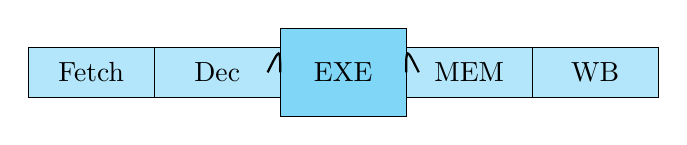
\begin{tikzpicture}[scale=0.8]
      % Single pipeline with bulge at EXE
      \draw[fill=cyan!30] (0,0) rectangle (2,0.8) node[midway] {Fetch};
      \draw[fill=cyan!30] (2,0) rectangle (4,0.8) node[midway] {Dec};
      \draw[fill=cyan!50] (4,-0.3) rectangle (6,1.1);
      \node at (5,0.4) {EXE};
      \draw[fill=cyan!30] (6,0) rectangle (8,0.8) node[midway] {MEM};
      \draw[fill=cyan!30] (8,0) rectangle (10,0.8) node[midway] {WB};
      
      % Curved lines showing bottleneck
      \draw[thick] (3.8,0.4) .. controls (4,0.8) and (4,0.8) .. (4,0.4);
      \draw[thick] (6,0.4) .. controls (6,0.8) and (6,0.8) .. (6.2,0.4);
    \end{tikzpicture}
  \end{center}
  
  \vspace{0.3cm}
  \begin{itemize}
    \item \textbf{Getting IPC $> 1$ requires to fetch, decode, exe, and retire $>1$ instruction per clock:}
  \end{itemize}
  
  \begin{center}
    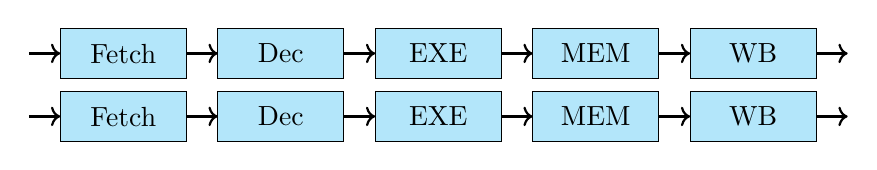
\begin{tikzpicture}[scale=0.8]
      % Dual pipeline
      \foreach \y in {0, -1} {
        \draw[->, thick] (-0.5,\y+0.4) -- (0,\y+0.4);
        \draw[fill=cyan!30] (0,\y) rectangle (2,\y+0.8) node[midway] {Fetch};
        \draw[->, thick] (2,\y+0.4) -- (2.5,\y+0.4);
        \draw[fill=cyan!30] (2.5,\y) rectangle (4.5,\y+0.8) node[midway] {Dec};
        \draw[->, thick] (4.5,\y+0.4) -- (5,\y+0.4);
        \draw[fill=cyan!30] (5,\y) rectangle (7,\y+0.8) node[midway] {EXE};
        \draw[->, thick] (7,\y+0.4) -- (7.5,\y+0.4);
        \draw[fill=cyan!30] (7.5,\y) rectangle (9.5,\y+0.8) node[midway] {MEM};
        \draw[->, thick] (9.5,\y+0.4) -- (10,\y+0.4);
        \draw[fill=cyan!30] (10,\y) rectangle (12,\y+0.8) node[midway] {WB};
        \draw[->, thick] (12,\y+0.4) -- (12.5,\y+0.4);
      }
    \end{tikzpicture}
  \end{center}
\end{frame}

\begin{frame}{The Pentium® Processor (1993)}
  \begin{itemize}
    \item \textbf{Fetch and decode 2 instructions per cycle}
    
    \item \textbf{At decode stage decide on \emph{pairing}:} can the two instructions be executed in parallel
    
    \item \textbf{Pairing decision is based on:}
    \begin{itemize}
      \item \textcolor{blue}{Data dependencies}: 2nd instruction must be independent of 1st
      \begin{itemize}
        \item If the 1st instruction produces data needed by the 2nd instruction, the 2nd instruction cannot be executed in parallel to the 1st instruction
      \end{itemize}
      
      \item \textcolor{blue}{Resources}: U-pipe and V-pipe are not symmetric (save HW)
      \begin{itemize}
        \item Common instructions can execute on either pipe
        \item Some instructions can execute only on the U-pipe
        \item V-pipe can run a subset of the instructions that can run on U-pipe
        \item If the 2nd instruction requires the U-pipe, it cannot pair
        \item Some instructions use resources of both pipes (and therefore cannot pair)
      \end{itemize}
    \end{itemize}
  \end{itemize}
  
  \begin{center}
    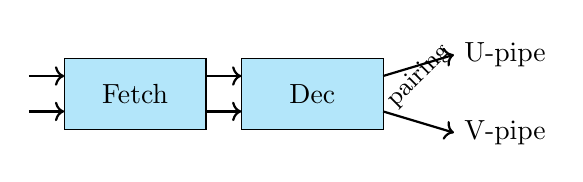
\begin{tikzpicture}[scale=0.9]
      \draw[->, thick] (-0.5,0) -- (0,0);
      \draw[->, thick] (-0.5,-0.5) -- (0,-0.5);
      \draw[fill=cyan!30] (0,-0.75) rectangle (2,0.25) node[midway] {Fetch};
      \draw[->, thick] (2,0) -- (2.5,0);
      \draw[->, thick] (2,-0.5) -- (2.5,-0.5);
      \draw[fill=cyan!30] (2.5,-0.75) rectangle (4.5,0.25) node[midway] {Dec};
      \node[rotate=45] at (5,0) {\small pairing};
      \draw[->, thick] (4.5,0) -- (5.5,0.3) node[right] {U-pipe};
      \draw[->, thick] (4.5,-0.5) -- (5.5,-0.8) node[right] {V-pipe};
    \end{tikzpicture}
  \end{center}
\end{frame}

\begin{frame}{Misprediction Penalty in a Superscalar CPU}
  \begin{itemize}
    \item \textbf{Assume}
    \begin{itemize}
      \item $\frac{1}{100}$ instruction is a mispredicted jump (MPI = 1\%)
      \item Flush penalty of 5 cycles
    \end{itemize}
    
    \vspace{0.5cm}
    
    \item \textbf{For IPC = 2}
    \begin{itemize}
      \item Flush every $\frac{100}{2} = 50$ cycles
      \item 5 cycles flush penalty every 50 cycles $\Rightarrow$ \alert{10\% performance hit}
    \end{itemize}
    
    \vspace{0.5cm}
    
    \item \textbf{For IPC = 1}
    \begin{itemize}
      \item Flush every $\frac{100}{1} = 100$ cycles
      \item 5 cycles flush penalty per 100 cycles $\Rightarrow$ \alert{5\% performance hit}
    \end{itemize}
    
    \vspace{0.5cm}
    
    \item \alert{Flush penalty increases as the machine is deeper and wider}
  \end{itemize}
\end{frame}

\begin{frame}{Extract More ILP}
  \begin{itemize}
    \item \textbf{ILP -- Instruction Level Parallelism}
    \begin{itemize}
      \item A given program, executed on a given input data has a given parallelism
      \item Can execute only independent instructions in parallel
      \item If for example each instruction is dependent on the previous instruction, ILP = 1
      \begin{itemize}
        \item Adding more HW will not change that
      \end{itemize}
    \end{itemize}
    
    \item \textbf{Adjacent instructions are usually dependent}
    \begin{itemize}
      \item 2nd pipe utilization is lower than 1st pipe utilization, a 3rd pipe utilization further goes down
    \end{itemize}
    
    \item \textbf{Cache misses stall execution} -- instructions dependent on a missed load stall
    
    \item \textbf{Compilers are limited to basic blocks}, and are not aware of cache misses
    
    \item \textbf{Solution: Out-Of-Order Execution}
    \begin{itemize}
      \item Look for independent instructions further ahead in the program
      \item Execute instructions based on data readiness
      \item Still need to keep the semantics of the original program
    \end{itemize}
  \end{itemize}
\end{frame}

\begin{frame}{Data Flow Analysis}
  \begin{columns}
    \begin{column}{0.35\textwidth}
      \textbf{Example:}
      \begin{enumerate}
        \item \texttt{\textcolor{r1color}{r1} $\leftarrow$ r4 / r7}
        \item \texttt{\textcolor{r8color}{r8} $\leftarrow$ \textcolor{r1color}{r1} + r2}
        \item \texttt{\textcolor{r5color}{r5} $\leftarrow$ r5 + 1}
        \item \texttt{\textcolor{r6color}{r6} $\leftarrow$ r6 - r3}
        \item \texttt{\textcolor{r4color}{r4} $\leftarrow$ \textcolor{r5color}{r5} + \textcolor{r6color}{r6}}
        \item \texttt{r7 $\leftarrow$ \textcolor{r8color}{r8} * \textcolor{r4color}{r4}}
      \end{enumerate}
      
      \vspace{0.3cm}
      \small{Assume divide takes multiple cycles}
    \end{column}
    
    \begin{column}{0.65\textwidth}
      \begin{center}
        \textbf{Data Flow Graph}\\
        \vspace{0.3cm}
        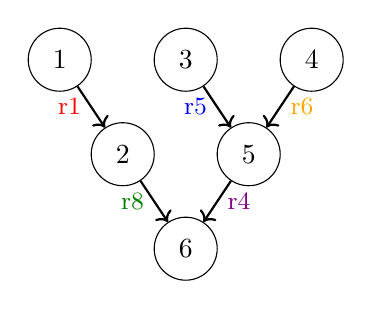
\begin{tikzpicture}[scale=0.8, 
          node distance=1.2cm,
          inst/.style={circle, draw, minimum size=0.8cm},
          dep/.style={->, thick}]
          
          % Nodes
          \node[inst] (i1) at (0,2.5) {1};
          \node[inst] (i3) at (2,2.5) {3};
          \node[inst] (i4) at (4,2.5) {4};
          \node[inst] (i2) at (1,1) {2};
          \node[inst] (i5) at (3,1) {5};
          \node[inst] (i6) at (2,-0.5) {6};
          
          % Dependencies with colored labels
          \draw[dep] (i1) -- node[left] {\textcolor{r1color}{\small r1}} (i2);
          \draw[dep] (i3) -- node[left] {\textcolor{r5color}{\small r5}} (i5);
          \draw[dep] (i4) -- node[right] {\textcolor{r6color}{\small r6}} (i5);
          \draw[dep] (i2) -- node[left] {\textcolor{r8color}{\small r8}} (i6);
          \draw[dep] (i5) -- node[right] {\textcolor{r4color}{\small r4}} (i6);
        \end{tikzpicture}
        
        \vspace{0.5cm}
        \small
        \begin{tabular}{cc}
          \textbf{In-order execution} & \textbf{Out-of-order execution} \\
        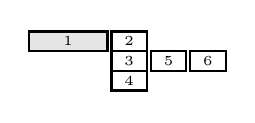
\begin{tikzpicture}[scale=0.5]
        % Box 1 (large, left side)
        \draw[thick, fill=gray!20] (0,1) rectangle (2,1.5) node[midway, font=\tiny] {1};
        
        % Box 2 (top right)
        \draw[thick, fill=white] (2.1,1) rectangle (3,1.5) node[midway, font=\tiny] {2};
        
        % Box 3 (middle right)
        \draw[thick, fill=white] (2.1,0.5) rectangle (3,1) node[midway, font=\tiny] {3};
        
        % Box 4 (bottom middle)
        \draw[thick, fill=white] (2.1,0) rectangle (3,0.5) node[midway, font=\tiny] {4};
        
        % Box 5 (right of box 3)
        \draw[thick, fill=white] (3.1,0.5) rectangle (4,1) node[midway, font=\tiny] {5};
        
        % Box 6 (far right)
        \draw[thick, fill=white] (4.1,0.5) rectangle (5,1) node[midway, font=\tiny] {6};
        \end{tikzpicture}
          &
          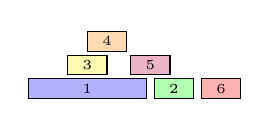
\begin{tikzpicture}[scale=0.5]
            \draw[fill=blue!30] (0,0) rectangle (3,0.5) node[midway] {\tiny 1};
            \draw[fill=yellow!30] (1,0.6) rectangle (2,1.1) node[midway] {\tiny 3};
            \draw[fill=orange!30] (1.5,1.2) rectangle (2.5,1.7) node[midway] {\tiny 4};
            \draw[fill=purple!30] (2.6,0.6) rectangle (3.6,1.1) node[midway] {\tiny 5};
            \draw[fill=green!30] (3.2,0) rectangle (4.2,0.5) node[midway] {\tiny 2};
            \draw[fill=red!30] (4.4,0) rectangle (5.4,0.5) node[midway] {\tiny 6};
          \end{tikzpicture}
        \end{tabular}
      \end{center}
    \end{column}
  \end{columns}
\end{frame}

\begin{frame}{OOOE: General Scheme}
  \begin{center}
    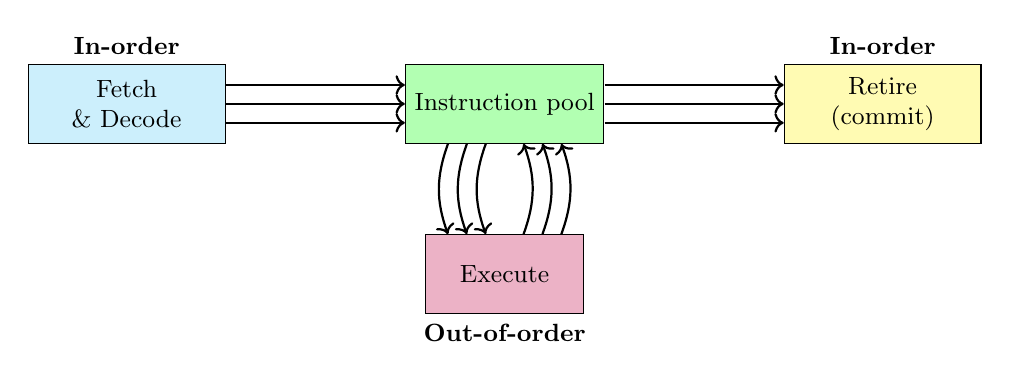
\begin{tikzpicture}[scale=1.2, every node/.style={font=\small},
      fetchblock/.style={rectangle, draw, fill=cyan!20, minimum width=2.5cm, minimum height=1cm},
      block/.style={rectangle, draw, fill=yellow!30, minimum width=2.5cm, minimum height=1cm},
      pool/.style={rectangle, draw, fill=green!30, minimum width=2.5cm, minimum height=1cm},
      exe/.style={rectangle, draw, fill=purple!30, minimum width=2cm, minimum height=1cm}]

      % Blocks
      \node[fetchblock,align=center] (fetch) at (0,0) {Fetch \\\& Decode};
      \node[pool] (pool) at (4,0) {Instruction pool};
      \node[exe] (exec) at (4,-1.8) {Execute};
      \node[block,align=center] (retire) at (8,0) {Retire\\(commit)};
      
      % Arrows with multiple lines
      \draw[->, thick] ([yshift=2mm]fetch.east) -- ([yshift=2mm]pool.west);
      \draw[->, thick] (fetch.east) -- (pool.west);
      \draw[->, thick] ([yshift=-2mm]fetch.east) -- ([yshift=-2mm]pool.west);

      \foreach \y in {-2mm, 0, 2mm} {
        \draw[->, thick] ([yshift=\y]pool.east) -- ([yshift=\y]retire.west);
      }
      
      % Bidirectional connection pool-execute
      \foreach \x in {-6mm, -4mm, -2mm} {
        \draw[->, thick, bend right=20] ([xshift=\x]pool.south) to ([xshift=\x]exec.north);
      }
      \foreach \x in {6mm, 4mm, 2mm} {
        \draw[<-, thick, bend left=20] ([xshift=\x]pool.south) to ([xshift=\x]exec.north);
      }
      % Labels
      \node[above] at (fetch.north) {\textbf{In-order}};
      \node[above] at (retire.north) {\textbf{In-order}};
      \node[below] at (exec.south) {\textbf{Out-of-order}};
    \end{tikzpicture}
  \end{center}
  
  \vspace{0.5cm}
  
  \begin{itemize}
    \item \textbf{Fetch \& decode instructions in parallel but in-order}
    \begin{itemize}
      \item Fill the Instruction Pool
    \end{itemize}
    
    \item \textbf{Execute ready instructions from the instructions pool}
    \begin{itemize}
      \item All source data ready + needed execution resources available
    \end{itemize}
    
    \item \textbf{Once an instruction is executed}
    \begin{itemize}
      \item Signal all dependent instructions that data is ready
    \end{itemize}
    
    \item \textbf{Commit instructions in parallel but in-order}
    \begin{itemize}
      \item State change (memory, register) and fault/exception handling
    \end{itemize}
  \end{itemize}
\end{frame}

\begin{frame}{Write-After-Write Dependency}
  \begin{columns}
    \begin{column}{0.5\textwidth}
      \textbf{Example Code:} \\
      \begin{tabular}{lll}
        (1) & & \texttt{\textcolor{r1color}{r1} $\leftarrow$ r9/17} \\
        (2) & & \texttt{\textcolor{r2color}{r2} $\leftarrow$ \textcolor{r2color}{r2}+\textcolor{r1color}{r1}} \\
        (3) & & \texttt{\textcolor{orange}{r1} $\leftarrow$ 23} \\
        (4) & & \texttt{\textcolor{r3color}{r3} $\leftarrow$ \textcolor{r3color}{r3}+\textcolor{orange}{r1}} \\
        (5) & & \texttt{jcc L2} \\
        (6) & \texttt{L2:} & \texttt{\textcolor{green}{r1} $\leftarrow$ 35} \\
        (7) & & \texttt{\textcolor{r4color}{r4} $\leftarrow$ \textcolor{r3color}{r3}+\textcolor{green}{r1}} \\
        (8) & & \texttt{\textcolor{blue}{r3} $\leftarrow$ 2} \\
      \end{tabular}
    \end{column}
    
    \begin{column}{0.5\textwidth}
      \begin{block}{WAW Issue}
        If inst (3) is executed before inst (1), r1 ends up having a wrong value.
        
        \vspace{0.3cm}
        
        Called \alert{write-after-write false dependency}:
        
        The order of two writes to the same register is flipped.
      \end{block}
    \end{column}
  \end{columns}
\end{frame}
\begin{frame}{What's Next}
  \begin{itemize}
    \item \textbf{Goal: minimize CPU Time}
    \begin{equation*}
      \text{CPU Time} = \text{clock cycle} \times \text{CPI} \times \text{IC}
    \end{equation*}
    
    \item \textbf{So far we have learned}
    \begin{itemize}
      \item Minimize clock cycle $\Rightarrow$ add more pipe stages
      \item Minimize CPI $\Rightarrow$ use pipeline
      \item Minimize IC $\Rightarrow$ architecture
    \end{itemize}
    
    \item \textbf{In a pipelined CPU}
    \begin{itemize}
      \item CPI w/o hazards is 1
      \item CPI with hazards is $> 1$
    \end{itemize}
    
    \item \textbf{Adding more pipe stages reduces clock cycle but increases CPI}
    \begin{itemize}
      \item Higher penalty due to control hazards
      \item More data hazards
    \end{itemize}
    
    \item \alert{What can we do? Further reduce the CPI!}
  \end{itemize}
\end{frame}

\begin{frame}{A Superscalar CPU}
  \begin{itemize}
    \item \textbf{Duplicating HW in one pipe stage won't help}
    \begin{itemize}
      \item e.g., have 2 ALUs
      \item the bottleneck moves to other stages
    \end{itemize}
  \end{itemize}
  
  \begin{center}
    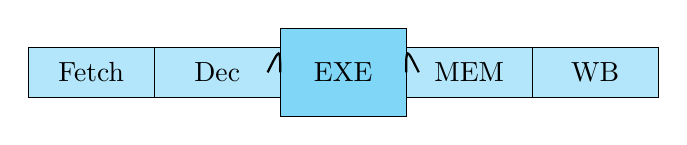
\begin{tikzpicture}[scale=0.8]
      % Single pipeline with bulge at EXE
      \draw[fill=cyan!30] (0,0) rectangle (2,0.8) node[midway] {Fetch};
      \draw[fill=cyan!30] (2,0) rectangle (4,0.8) node[midway] {Dec};
      \draw[fill=cyan!50] (4,-0.3) rectangle (6,1.1);
      \node at (5,0.4) {EXE};
      \draw[fill=cyan!30] (6,0) rectangle (8,0.8) node[midway] {MEM};
      \draw[fill=cyan!30] (8,0) rectangle (10,0.8) node[midway] {WB};
      
      % Curved lines showing bottleneck
      \draw[thick] (3.8,0.4) .. controls (4,0.8) and (4,0.8) .. (4,0.4);
      \draw[thick] (6,0.4) .. controls (6,0.8) and (6,0.8) .. (6.2,0.4);
    \end{tikzpicture}
  \end{center}
  
  \vspace{0.3cm}
  \begin{itemize}
    \item \textbf{Getting IPC $> 1$ requires to fetch, decode, exe, and retire $>1$ instruction per clock:}
  \end{itemize}
  
  \begin{center}
    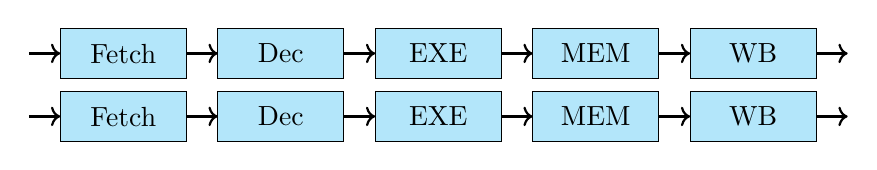
\begin{tikzpicture}[scale=0.8]
      % Dual pipeline
      \foreach \y in {0, -1} {
        \draw[->, thick] (-0.5,\y+0.4) -- (0,\y+0.4);
        \draw[fill=cyan!30] (0,\y) rectangle (2,\y+0.8) node[midway] {Fetch};
        \draw[->, thick] (2,\y+0.4) -- (2.5,\y+0.4);
        \draw[fill=cyan!30] (2.5,\y) rectangle (4.5,\y+0.8) node[midway] {Dec};
        \draw[->, thick] (4.5,\y+0.4) -- (5,\y+0.4);
        \draw[fill=cyan!30] (5,\y) rectangle (7,\y+0.8) node[midway] {EXE};
        \draw[->, thick] (7,\y+0.4) -- (7.5,\y+0.4);
        \draw[fill=cyan!30] (7.5,\y) rectangle (9.5,\y+0.8) node[midway] {MEM};
        \draw[->, thick] (9.5,\y+0.4) -- (10,\y+0.4);
        \draw[fill=cyan!30] (10,\y) rectangle (12,\y+0.8) node[midway] {WB};
        \draw[->, thick] (12,\y+0.4) -- (12.5,\y+0.4);
      }
    \end{tikzpicture}
  \end{center}
\end{frame}

\begin{frame}{The Pentium® Processor (1993)}
  \begin{itemize}
    \item \textbf{Fetch and decode 2 instructions per cycle}
    
    \item \textbf{At decode stage decide on \emph{pairing}:} can the two instructions be executed in parallel
    
    \item \textbf{Pairing decision is based on:}
    \begin{itemize}
      \item \textcolor{blue}{Data dependencies}: 2nd instruction must be independent of 1st
      \begin{itemize}
        \item If the 1st instruction produces data needed by the 2nd instruction, the 2nd instruction cannot be executed in parallel to the 1st instruction
      \end{itemize}
      
      \item \textcolor{blue}{Resources}: U-pipe and V-pipe are not symmetric (save HW)
      \begin{itemize}
        \item Common instructions can execute on either pipe
        \item Some instructions can execute only on the U-pipe
        \item V-pipe can run a subset of the instructions that can run on U-pipe
        \item If the 2nd instruction requires the U-pipe, it cannot pair
        \item Some instructions use resources of both pipes (and therefore cannot pair)
      \end{itemize}
    \end{itemize}
  \end{itemize}
  
  \begin{center}
    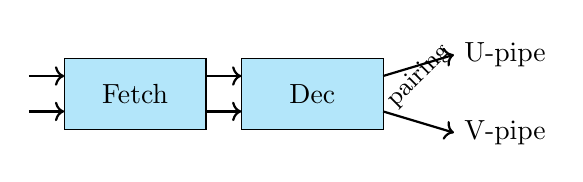
\begin{tikzpicture}[scale=0.9]
      \draw[->, thick] (-0.5,0) -- (0,0);
      \draw[->, thick] (-0.5,-0.5) -- (0,-0.5);
      \draw[fill=cyan!30] (0,-0.75) rectangle (2,0.25) node[midway] {Fetch};
      \draw[->, thick] (2,0) -- (2.5,0);
      \draw[->, thick] (2,-0.5) -- (2.5,-0.5);
      \draw[fill=cyan!30] (2.5,-0.75) rectangle (4.5,0.25) node[midway] {Dec};
      \node[rotate=45] at (5,0) {\small pairing};
      \draw[->, thick] (4.5,0) -- (5.5,0.3) node[right] {U-pipe};
      \draw[->, thick] (4.5,-0.5) -- (5.5,-0.8) node[right] {V-pipe};
    \end{tikzpicture}
  \end{center}
\end{frame}

\begin{frame}{Misprediction Penalty in a Superscalar CPU}
  \begin{itemize}
    \item \textbf{Assume}
    \begin{itemize}
      \item $\frac{1}{100}$ instruction is a mispredicted jump (MPI = 1\%)
      \item Flush penalty of 5 cycles
    \end{itemize}
    
    \vspace{0.5cm}
    
    \item \textbf{For IPC = 2}
    \begin{itemize}
      \item Flush every $\frac{100}{2} = 50$ cycles
      \item 5 cycles flush penalty every 50 cycles $\Rightarrow$ \alert{10\% performance hit}
    \end{itemize}
    
    \vspace{0.5cm}
    
    \item \textbf{For IPC = 1}
    \begin{itemize}
      \item Flush every $\frac{100}{1} = 100$ cycles
      \item 5 cycles flush penalty per 100 cycles $\Rightarrow$ \alert{5\% performance hit}
    \end{itemize}
    
    \vspace{0.5cm}
    
    \item \alert{Flush penalty increases as the machine is deeper and wider}
  \end{itemize}
\end{frame}

\begin{frame}{Extract More ILP}
  \begin{itemize}
    \item \textbf{ILP -- Instruction Level Parallelism}
    \begin{itemize}
      \item A given program, executed on a given input data has a given parallelism
      \item Can execute only independent instructions in parallel
      \item If for example each instruction is dependent on the previous instruction, ILP = 1
      \begin{itemize}
        \item Adding more HW will not change that
      \end{itemize}
    \end{itemize}
    
    \item \textbf{Adjacent instructions are usually dependent}
    \begin{itemize}
      \item 2nd pipe utilization is lower than 1st pipe utilization, a 3rd pipe utilization further goes down
    \end{itemize}
    
    \item \textbf{Cache misses stall execution} -- instructions dependent on a missed load stall
    
    \item \textbf{Compilers are limited to basic blocks}, and are not aware of cache misses
    
    \item \textbf{Solution: Out-Of-Order Execution}
    \begin{itemize}
      \item Look for independent instructions further ahead in the program
      \item Execute instructions based on data readiness
      \item Still need to keep the semantics of the original program
    \end{itemize}
  \end{itemize}
\end{frame}

\begin{frame}{Data Flow Analysis}
  \begin{columns}
    \begin{column}{0.35\textwidth}
      \textbf{Example:}
      \begin{enumerate}
        \item \texttt{\textcolor{r1color}{r1} $\leftarrow$ r4 / r7}
        \item \texttt{\textcolor{r8color}{r8} $\leftarrow$ \textcolor{r1color}{r1} + r2}
        \item \texttt{\textcolor{r5color}{r5} $\leftarrow$ r5 + 1}
        \item \texttt{\textcolor{r6color}{r6} $\leftarrow$ r6 - r3}
        \item \texttt{\textcolor{r4color}{r4} $\leftarrow$ \textcolor{r5color}{r5} + \textcolor{r6color}{r6}}
        \item \texttt{r7 $\leftarrow$ \textcolor{r8color}{r8} * \textcolor{r4color}{r4}}
      \end{enumerate}
      
      \vspace{0.3cm}
      \small{Assume divide takes multiple cycles}
    \end{column}
    
    \begin{column}{0.65\textwidth}
      \begin{center}
        \textbf{Data Flow Graph}\\
        \vspace{0.3cm}
        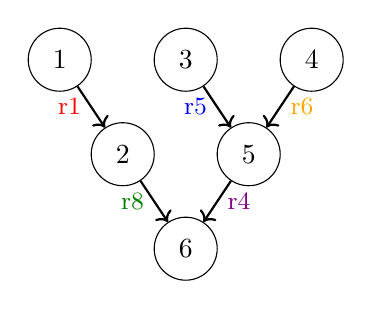
\begin{tikzpicture}[scale=0.8, 
          node distance=1.2cm,
          inst/.style={circle, draw, minimum size=0.8cm},
          dep/.style={->, thick}]
          
          % Nodes
          \node[inst] (i1) at (0,2.5) {1};
          \node[inst] (i3) at (2,2.5) {3};
          \node[inst] (i4) at (4,2.5) {4};
          \node[inst] (i2) at (1,1) {2};
          \node[inst] (i5) at (3,1) {5};
          \node[inst] (i6) at (2,-0.5) {6};
          
          % Dependencies with colored labels
          \draw[dep] (i1) -- node[left] {\textcolor{r1color}{\small r1}} (i2);
          \draw[dep] (i3) -- node[left] {\textcolor{r5color}{\small r5}} (i5);
          \draw[dep] (i4) -- node[right] {\textcolor{r6color}{\small r6}} (i5);
          \draw[dep] (i2) -- node[left] {\textcolor{r8color}{\small r8}} (i6);
          \draw[dep] (i5) -- node[right] {\textcolor{r4color}{\small r4}} (i6);
        \end{tikzpicture}
        
        \vspace{0.5cm}
        \small
        \begin{tabular}{cc}
          \textbf{In-order execution} & \textbf{Out-of-order execution} \\
        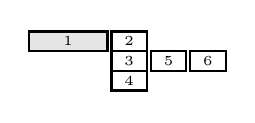
\begin{tikzpicture}[scale=0.5]
        % Box 1 (large, left side)
        \draw[thick, fill=gray!20] (0,1) rectangle (2,1.5) node[midway, font=\tiny] {1};
        
        % Box 2 (top right)
        \draw[thick, fill=white] (2.1,1) rectangle (3,1.5) node[midway, font=\tiny] {2};
        
        % Box 3 (middle right)
        \draw[thick, fill=white] (2.1,0.5) rectangle (3,1) node[midway, font=\tiny] {3};
        
        % Box 4 (bottom middle)
        \draw[thick, fill=white] (2.1,0) rectangle (3,0.5) node[midway, font=\tiny] {4};
        
        % Box 5 (right of box 3)
        \draw[thick, fill=white] (3.1,0.5) rectangle (4,1) node[midway, font=\tiny] {5};
        
        % Box 6 (far right)
        \draw[thick, fill=white] (4.1,0.5) rectangle (5,1) node[midway, font=\tiny] {6};
        \end{tikzpicture}
          &
          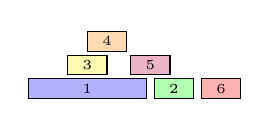
\begin{tikzpicture}[scale=0.5]
            \draw[fill=blue!30] (0,0) rectangle (3,0.5) node[midway] {\tiny 1};
            \draw[fill=yellow!30] (1,0.6) rectangle (2,1.1) node[midway] {\tiny 3};
            \draw[fill=orange!30] (1.5,1.2) rectangle (2.5,1.7) node[midway] {\tiny 4};
            \draw[fill=purple!30] (2.6,0.6) rectangle (3.6,1.1) node[midway] {\tiny 5};
            \draw[fill=green!30] (3.2,0) rectangle (4.2,0.5) node[midway] {\tiny 2};
            \draw[fill=red!30] (4.4,0) rectangle (5.4,0.5) node[midway] {\tiny 6};
          \end{tikzpicture}
        \end{tabular}
      \end{center}
    \end{column}
  \end{columns}
\end{frame}

\begin{frame}{Write-After-Write Dependency}
  \begin{columns}
    \begin{column}{0.5\textwidth}
      \textbf{Example Code:} \\
      \begin{tabular}{lll}
        (1) & & \texttt{\textcolor{blue}{r1} $\leftarrow$ r9/17} \\
        (2) & & \texttt{r2 $\leftarrow$ r2+\textcolor{blue}{r1}} \\
        (3) & & \texttt{\textcolor{orange}{r1} $\leftarrow$ 23} \\
        (4) & & \texttt{r3 $\leftarrow$ r3+\textcolor{orange}{r1}} \\
        (5) & & \texttt{jcc L2} \\
        (6) & \texttt{L2:} & \texttt{\textcolor{green}{r1} $\leftarrow$ 35} \\
        (7) & & \texttt{r4 $\leftarrow$ r3+\textcolor{green}{r1}} \\
        (8) & & \texttt{r3 $\leftarrow$ 2} \\
      \end{tabular}
    \end{column}
    
    \begin{column}{0.5\textwidth}
      \begin{block}{WAW Issue}
        If inst (3) is executed before inst (1), r1 ends up having a wrong value.
        
        \vspace{0.3cm}
        
        Called \alert{write-after-write false dependency}:
        
        The order of two writes to the same register is flipped.
      \end{block}
    \end{column}
  \end{columns}
\end{frame}

\begin{frame}{WAW False Dependency}
  \begin{columns}
    \begin{column}{0.5\textwidth}
      \textbf{Example Code (reordered):} \\
      \begin{tabular}{lll}
        (3) & & \texttt{\textcolor{orange}{r1\tikzmark{r1dest}} $\leftarrow$ 23} \\
        (1) & & \texttt{\textcolor{blue}{r1\tikzmark{r1blue}} $\leftarrow$ r9/17} \\
        (2) & & \texttt{r2 $\leftarrow$ r2+\textcolor{blue}{r1}} \\
        & & \\
        (4) & & \texttt{r3 $\leftarrow$ r3+\textcolor{orange}{\tikzmark{r1use}r1}} \\
        (5) & & \texttt{jcc L2} \\
        (6) & \texttt{L2:} & \texttt{\textcolor{green}{r1} $\leftarrow$ 35} \\
        (7) & & \texttt{r4 $\leftarrow$ r3+\textcolor{green}{r1}} \\
        (8) & & \texttt{r3 $\leftarrow$ 2} \\
      \end{tabular}
    \end{column}

    \begin{column}{0.5\textwidth}
      % Arrow showing dependency using tikzmark and callout
      \begin{tikzpicture}[overlay, remember picture]
        \draw[->, thick, orange, dashed] ([xshift=0mm, yshift=1mm]pic cs:r1dest) to[out=0, in=90] ([xshift=2mm, yshift=3mm]pic cs:r1use);
        \draw[->, thick, blue] ([xshift=0mm, yshift=1mm]pic cs:r1blue) -- ([xshift=0mm, yshift=3mm]pic cs:r1use);

        % Callout for specific example positioned relative to r1dest
        \node[rectangle callout, draw=orange, fill=orange!10, thick, align=left, text width=4.5cm,
              font=\small, anchor=west, callout absolute pointer={([xshift=5mm, yshift=2mm]pic cs:r1use)}]
          at ([xshift=3.5cm, yshift=1.3cm]pic cs:r1use)
          {Instruction (4) must use \textcolor{orange}{r1} from instruction (3), not from instruction (1)};
      \end{tikzpicture}

      \vspace{3cm}

      \pause

      \begin{alertblock}{Write-After-Write (WAW)}
        \alert{WAW is a \emph{false dependency}}

        \vspace{0.2cm}

        Not a real data dependency, but an artifact of OOO execution when multiple writes target the same register.
      \end{alertblock}
    \end{column}
  \end{columns}
\end{frame}

\begin{frame}{Speculative Execution}
  \begin{columns}
    \begin{column}{0.45\textwidth}
      \textbf{Example Code:} \\
      \begin{tabular}{lll}
        (3) & & \texttt{\textcolor{orange}{r1} $\leftarrow$ 23} \\
        (1) & & \texttt{\textcolor{blue}{r1} $\leftarrow$ r9/17} \\
        (2) & & \texttt{r2 $\leftarrow$ r2+\textcolor{blue}{r1}} \\
        (4) & & \texttt{r3 $\leftarrow$ r3+\textcolor{orange}{r1}} \\
        (5) & & \texttt{jcc L2} \\
        \rowcolor{pink!30} (6) & \texttt{L2:} & \texttt{\textcolor{green}{r1} $\leftarrow$ 35} \\
        \rowcolor{pink!30} (7) & & \texttt{r4 $\leftarrow$ r3+\textcolor{green}{r1}} \\
        \rowcolor{pink!30} (8) & & \texttt{r3 $\leftarrow$ 2} \\
      \end{tabular}
    \end{column}
    
    \begin{column}{0.55\textwidth}
      \begin{block}{OOO Speculative Execution}
        \small
        \textbf{Every 5th instruction is a branch} $\Rightarrow$ must continue fetching along \textcolor{green}{predicted path} to fill instruction pool.
        
        Without speculation: limited to finding independent instructions only until next branch.
        
        \alert{Speculative Execution:} Execute instructions from predicted path before branch resolution.
        
        Example: inst (6) can execute before inst (1).
        
        If mispredicted: must undo speculatively executed instructions.
      \end{block}
    \end{column}
  \end{columns}
\end{frame}

\begin{frame}{WAR False Dependency}
  \begin{columns}
    \begin{column}{0.5\textwidth}
      \textbf{Example Code (reordered):} \\
      \begin{tabular}{lll}
        (3) & & \texttt{\textcolor{orange}{r1} $\leftarrow$ 23} \\
        (1) & & \texttt{\textcolor{blue}{r1} $\leftarrow$ r9/17} \\
        (2) & & \texttt{r2 $\leftarrow$ r2+\textcolor{blue}{r1}} \\
        & & \\
        (4) & & \texttt{r3 $\leftarrow$ r3+\textcolor{orange}{r1}} \\
        (5) & & \texttt{jcc L2} \\
        (6) & \texttt{L2:} & \texttt{\textcolor{green}{r1} $\leftarrow$ 35} \\
        (8) & & \texttt{\textcolor{blue}{r3\tikzmark{r3write}} $\leftarrow$ 2} \\
        (7) & & \texttt{r4 $\leftarrow$ \textcolor{red}{\tikzmark{r3read}r3}+\textcolor{green}{r1}} \\
      \end{tabular}
    \end{column}

    \begin{column}{0.5\textwidth}
      % Arrow showing dependency using tikzmark and callout
      \begin{tikzpicture}[overlay, remember picture]
        \draw[->, thick, blue] ([xshift=1mm, yshift=0mm]pic cs:r3write) -- ([xshift=-1mm, yshift=3mm]pic cs:r3read);

        % Callout for specific example positioned relative to r3read
        \node[rectangle callout, draw=red, fill=red!10, thick, align=left, text width=4.5cm,
              font=\small, anchor=west, callout absolute pointer={([xshift=5mm, yshift=2mm]pic cs:r3read)}]
          at ([xshift=4cm, yshift=4.5cm]pic cs:r3read)
          {Instruction (7) must read \textcolor{red}{r3} before instruction (8) overwrites it};
      \end{tikzpicture}

      \vspace{3cm}

      \pause

      \begin{alertblock}{Write-After-Read (WAR)}
        \alert{WAR is a \emph{false dependency}}

        \vspace{0.2cm}

        Not a real data dependency, but an artifact of OOO execution when a write happens before a read of the old value.
      \end{alertblock}
    \end{column}
  \end{columns}
\end{frame}

\begin{frame}{Register Renaming: Overview}
  \begin{itemize}
    \item \textbf{Physical register pool:} Maps architectural registers to physical registers
    
    \item \textbf{Allocation (in-order):}
    \begin{enumerate}
      \item If instruction writes Rx $\rightarrow$ allocate free physical register PRi
      \item Update mapping: Rx $\mapsto$ PRi
      \item Rename sources to their mapped physical registers
    \end{enumerate}
    
    \item \textbf{Execution (out-of-order):}
    \begin{itemize}
      \item Execute when sources ready \& resources available
      \item Write result to PRi (not Rx)
    \end{itemize}
    
    \item \textbf{Commit (in-order):}
    \begin{itemize}
      \item Copy PRi $\rightarrow$ Rx
      \item If Rx still maps to PRi: set mapping to architectural
      \item Return PRi to free pool
    \end{itemize}
  \end{itemize}
\end{frame}

\begin{frame}{Register Renaming: Example - Step 1}
  \begin{columns}[t]
    \begin{column}{0.5\textwidth}
      \begin{tabular}[t]{lll}
        \multicolumn{3}{c}{\textbf{Original}} \\
        (1) & r1 $\leftarrow$ 17 & \\
        (2) & r2 $\leftarrow$ r2+r1 & \\
        (3) & r1 $\leftarrow$ 23 & \\
        (4) & r3 $\leftarrow$ r3+r1 & \\
        (5) & jcc L2 & \\
        (6) L2: & r1 $\leftarrow$ 35 & \\
        (7) & r4 $\leftarrow$ r3+r1 & \\
        (8) & r3 $\leftarrow$ 2 & \\
      \end{tabular}
    \end{column}

    \begin{column}{0.5\textwidth}
      \begin{tabular}[t]{lll}
        \multicolumn{3}{c}{\textbf{Renaming}} \\
        r1:pr1 & pr1 $\leftarrow$ 17 & \\
        r2:pr2 & pr2 $\leftarrow$ r2+pr1 & \\
      \end{tabular}

      \vspace{0.3cm}
      \begin{block}{Note}
        \small
        When r2 is both source and destination: \textbf{read first} (using current mapping), then \textbf{write to new} physical register (update mapping).
      \end{block}
    \end{column}
  \end{columns}
  
  \vspace{0.3cm}
  \begin{center}
    \begin{tabular}{|c|c|c|c|c|}
      \hline
      & r1 & r2 & r3 & r4 \\
      \hline
      Register mapping & pr1 & pr2 & r3 & r4 \\
      \hline
    \end{tabular}
  \end{center}
\end{frame}

\begin{frame}{Register Renaming: Example - Step 2}
  \begin{columns}
    \begin{column}{0.5\textwidth}
      \begin{tabular}{lll}
        \multicolumn{3}{c}{\textbf{Original}} \\
        (1) & r1 $\leftarrow$ 17 & \\
        (2) & r2 $\leftarrow$ r2+r1 & \\
        (3) & r1 $\leftarrow$ 23 & \\
        (4) & r3 $\leftarrow$ r3+r1 & \\
        (5) & jcc L2 & \\
        (6) L2: & r1 $\leftarrow$ 35 & \\
        (7) & r4 $\leftarrow$ r3+r1 & \\
        (8) & r3 $\leftarrow$ 2 & \\
      \end{tabular}
    \end{column}

    \begin{column}{0.5\textwidth}
      \begin{tabular}{lll}
        \multicolumn{3}{c}{\textbf{Renaming}} \\
        r1:pr1 & pr1 $\leftarrow$ 17 & \\
        r2:pr2 & pr2 $\leftarrow$ r2+pr1 & \\
        r1:pr3 & pr3 $\leftarrow$ 23 & \\
        r3:pr4 & pr4 $\leftarrow$ r3+pr3 & \\
        & & \\
        & & \\
        & & \\
        & & \\
      \end{tabular}
    \end{column}
  \end{columns}

  \vspace{0.5cm}
  \begin{center}
    \begin{tabular}{|c|c|c|c|c|}
      \hline
      & r1 & r2 & r3 & r4 \\
      \hline
      Register mapping & pr3 & pr2 & pr4 & r4 \\
      \hline
    \end{tabular}
  \end{center}

  \begin{center}
    \colorbox{green!30}{Each instruction uses the correct sources, regardless of the execution order}
  \end{center}
\end{frame}

\begin{frame}{Register Renaming: Example - Complete}
  \begin{columns}
    \begin{column}{0.5\textwidth}
      \begin{tabular}{lll}
        \multicolumn{3}{c}{\textbf{Original}} \\
        (1) & r1 $\leftarrow$ 17 & \\
        (2) & r2 $\leftarrow$ r2+r1 & \\
        (3) & r1 $\leftarrow$ 23 & \\
        (4) & r3 $\leftarrow$ r3+r1 & \\
        (5) & jcc L2 & \\
        (6) L2: & r1 $\leftarrow$ 35 & \\
        (7) & r4 $\leftarrow$ r3+r1 & \\
        (8) & r3 $\leftarrow$ 2 & \\
      \end{tabular}
    \end{column}

    \begin{column}{0.5\textwidth}
      \begin{tabular}{lll}
        \multicolumn{3}{c}{\textbf{Renaming}} \\
        r1:pr1 & pr1 $\leftarrow$ 17 & \\
        r2:pr2 & pr2 $\leftarrow$ r2+pr1 & \\
        r1:pr3 & pr3 $\leftarrow$ 23 & \\
        r3:pr4 & pr4 $\leftarrow$ r3+pr3 & \\
        & & \\
        r1:pr5 & pr5 $\leftarrow$ 35 & \\
        r4:pr6 & pr6 $\leftarrow$ pr4+pr5 & \\
        r3:pr7 & pr7 $\leftarrow$ 2 & \\
      \end{tabular}
    \end{column}
  \end{columns}

  \vspace{0.5cm}
  \begin{center}
    \begin{tabular}{|c|c|c|c|c|}
      \hline
      & r1 & r2 & r3 & r4 \\
      \hline
      Register mapping & pr5 & pr2 & pr7 & pr6 \\
      \hline
    \end{tabular}
  \end{center}

  \begin{center}
    \colorbox{green!30}{Each instruction uses the correct sources, regardless of the execution order}
  \end{center}
\end{frame}

\begin{frame}{Speculative Execution -- Misprediction}
  \begin{columns}
    \begin{column}{0.5\textwidth}
      \begin{tabular}{lll}
        \multicolumn{3}{c}{\textbf{Original}} \\
        (1) & r1 $\leftarrow$ 17 & \\
        (2) & r2 $\leftarrow$ r2+r1 & \\
        (3) & r1 $\leftarrow$ 23 & \\
        (4) & r3 $\leftarrow$ r3+r1 & \\
        (5) & jcc L2 & \\
        \rowcolor{pink!30} (6) L2: & r1 $\leftarrow$ 35 & \\
        \rowcolor{pink!30} (7) & r4 $\leftarrow$ r3+r1 & \\
        \rowcolor{pink!30} (8) & r3 $\leftarrow$ 2 & \\
      \end{tabular}
    \end{column}
    
    \begin{column}{0.5\textwidth}
      \begin{tabular}{lll}
        \multicolumn{3}{c}{\textbf{Renaming}} \\
        r1:pr1 & pr1 $\leftarrow$ 17 & \\
        r2:pr2 & pr2 $\leftarrow$ r2+pr1 & \\
        r1:pr3 & pr3 $\leftarrow$ 23 & \\
        r3:pr4 & pr4 $\leftarrow$ r3+pr3 & \\
        & & \\
        \rowcolor{pink!30} r1:pr5 & pr5 $\leftarrow$ 35 & \\
        \rowcolor{pink!30} r4:pr6 & pr6 $\leftarrow$ pr4+pr5 & \\
        \rowcolor{pink!30} r3:pr7 & pr7 $\leftarrow$ 2 & \\
      \end{tabular}
    \end{column}
  \end{columns}
  
  \vspace{0.3cm}
  \begin{center}
    \begin{tabular}{|c|c|c|c|c|}
      \hline
      & r1 & r2 & r3 & r4 \\
      \hline
      Register mapping & pr3 & pr2 & pr4 & r4 \\
      \hline
    \end{tabular}
  \end{center}
  
  \begin{block}{Misprediction Recovery}
    If the predicted branch path turns out to be wrong (when the branch is executed):
    The instructions following the branch are flushed \textbf{before they are committed}
    $\Rightarrow$ the architectural state is not changed
  \end{block}
\end{frame}

\begin{frame}{Speculative Execution -- Misprediction}
  \begin{columns}
    \begin{column}{0.5\textwidth}
      \begin{tabular}{lll}
        \multicolumn{3}{c}{\textbf{Original}} \\
        (1) & r1 $\leftarrow$ 17 & \\
        (2) & r2 $\leftarrow$ r2+r1 & \\
        (3) & r1 $\leftarrow$ 23 & \\
        (4) & r3 $\leftarrow$ r3+r1 & \\
        (5) & jcc L2 & \\
        \rowcolor{pink!30} (6) L2: & r1 $\leftarrow$ 35 & \\
        \rowcolor{pink!30} (7) & r4 $\leftarrow$ r3+r1 & \\
        \rowcolor{pink!30} (8) & r3 $\leftarrow$ 2 & \\
      \end{tabular}
    \end{column}
    
    \begin{column}{0.5\textwidth}
      \begin{tabular}{lll}
        \multicolumn{3}{c}{\textbf{Renaming}} \\
        r1:pr1 & pr1 $\leftarrow$ 17 & \\
        r2:pr2 & pr2 $\leftarrow$ r2+pr1 & \\
        r1:pr3 & pr3 $\leftarrow$ 23 & \\
        r3:pr4 & pr4 $\leftarrow$ r3+pr3 & \\
        & & \\
        \rowcolor{pink!30} r1:pr5 & pr5 $\leftarrow$ 35 & \\
        \rowcolor{pink!30} r4:pr6 & pr6 $\leftarrow$ pr4+pr5 & \\
        \rowcolor{pink!30} r3:pr7 & pr7 $\leftarrow$ 2 & \\
      \end{tabular}
    \end{column}
  \end{columns}
  
  \vspace{0.3cm}
  \begin{center}
    \begin{tabular}{|c|c|c|c|c|}
      \hline
      & r1 & r2 & r3 & r4 \\
      \hline
      Register mapping & \textcolor{red}{\textcircled{pr5}} & pr2 & \textcolor{red}{\textcircled{pr7}} & \textcolor{red}{\textcircled{pr6}} \\
      \hline
    \end{tabular}
  \end{center}
  
  \begin{block}{Recovery Challenge}
    But the register mapping was already wrongly updated by the wrong path instructions
    
    \vspace{0.2cm}
    \colorbox{green!30}{Later on we will see various schemes for recovering the mapping}
  \end{block}
\end{frame}

\begin{frame}{A Superscalar OOO Machine}
  \begin{center}
    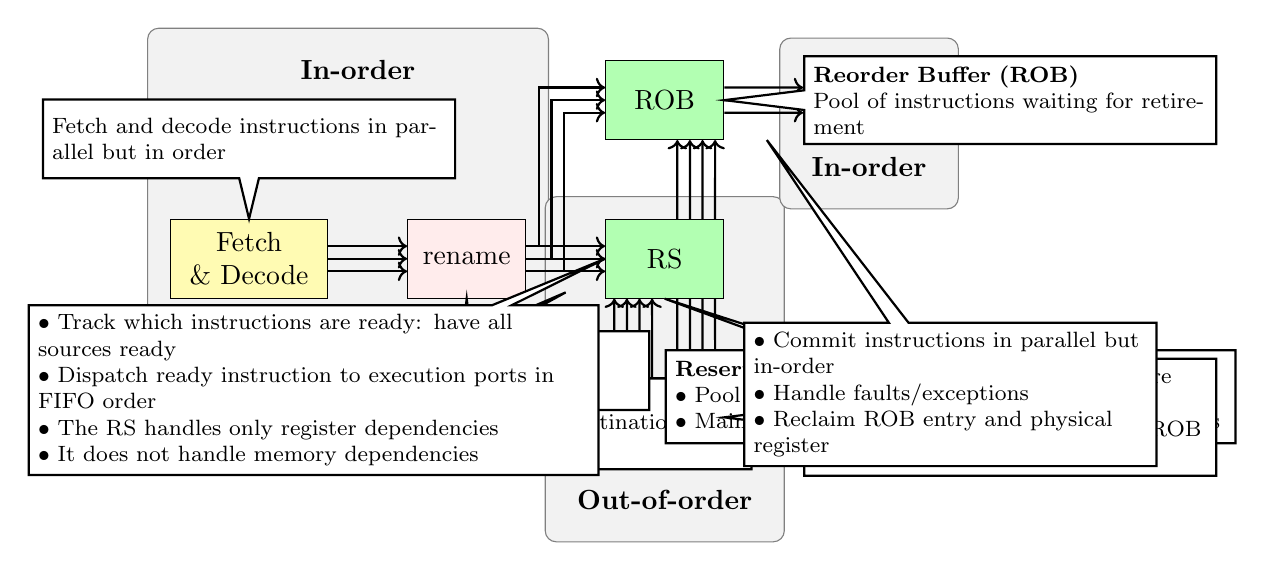
\begin{tikzpicture}[scale=0.8,
      node distance=1cm,
      block/.style={rectangle, draw, fill=yellow!30, minimum width=2cm, minimum height=1cm},
      rename/.style={rectangle, draw, fill=pink!30, minimum width=1.5cm, minimum height=1cm},
      pool/.style={rectangle, draw, fill=green!30, minimum width=1.5cm, minimum height=1cm},
      exe/.style={rectangle, draw, fill=purple!30, minimum width=1.5cm, minimum height=1cm},
      retire/.style={rectangle, draw, fill=yellow!30, minimum width=1.5cm, minimum height=1cm},
      calloutbox/.style={rectangle callout, draw, fill=white, thick, align=left,
                         text width=5cm, minimum height=1cm, font=\footnotesize},
      widecalloutbox/.style={calloutbox, text width=6cm},
      verywidecalloutbox/.style={calloutbox, text width=7cm}]

      % Stage 1: Fetch & Decode + rename
      \node[block,align=center] (fetch) at (0,0) {Fetch \\\& Decode};
      \node[rename, right=of fetch] (rename) {rename};

      % Stage 2: Add ROB and RS
      \onslide<2->{
        \node[pool, right=of rename] (rs) {RS};
        \node[pool, above=of rs] (rob) {ROB};
      }

      % Stage 3: Add Execute
      \onslide<3>{
        \node[exe, below=of rs] (execute) {Execute};
        \node[below=0.3cm of execute.south] (outoforder) {\textbf{Out-of-order}};
      }

      % Stage 4: Add Retire
      \onslide<4->{
        \node[retire,align=center, right=of rob] (retire) {Retire\\(commit)};
        \node[below=0.1cm of retire.south] (inorder2) {\textbf{In-order}};
      }

      % In-order label for initial stages
      \onslide<1-2>{
        \node at ($(fetch)!0.5!(rename)+(0,3)$)  (inorder) {\textbf{In-order}};
      }

      % Fit background for in-order section
      \onslide<1-2>{
        \node[draw=gray, fill=gray!10, fit=(fetch) (rename) (inorder), inner sep=8pt, rounded corners] (bg1) {};
      }
      \onslide<3>{
        \node[draw=gray, fill=gray!10, fit=(rs) (execute) (outoforder), inner sep=8pt, rounded corners] (bg2) {};
      }
      \onslide<4>{
        \node[draw=gray, fill=gray!10, fit=(retire) (inorder2), inner sep=8pt, rounded corners] (bg3) {};
      }

      % Redraw nodes on top to ensure they're visible
      \node[block,align=center] (fetch) at (0,0) {Fetch \\\& Decode};
      \node[rename, right=of fetch] (rename) {rename};
      \onslide<2->{
        \node[pool, right=of rename] (rs) {RS};
        \node[pool, above=of rs] (rob) {ROB};
      }
      \onslide<3->{
        \node[exe, below=of rs] (execute) {Execute};
      }
      \onslide<3>{
        \node[below=0.3cm of execute.south] (outoforder) {\textbf{Out-of-order}};
      }
      \onslide<4->{
        \node[retire,align=center, right=of rob] (retire) {Retire\\(commit)};
        \node[below=0.1cm of retire.south] (inorder2) {\textbf{In-order}};
      }
      \onslide<1-2>{
        \node at ($(fetch)!0.5!(rename)+(0,3)$)  (inorder) {\textbf{In-order}};
      }

      % Arrows - Stage 1
      \foreach \y in {-2mm, 0, 2mm} {
        \draw[->, thick] ([yshift=\y]fetch.east) -- ([yshift=\y]rename.west);
      }

      % Arrows - Stage 2
      \onslide<2->{
        \foreach \y in {-2mm, 0, 2mm} {
          \draw[->, thick] ([yshift=\y]rename.east) -- ([yshift=\y]rs.west);
        }
        \foreach \y in {-2mm, 0, 2mm} {
          \draw[->, thick] ([yshift=\y,xshift=-\y+4mm]rename.east) |- ([yshift=\y]rob.west);
        }
      }

      % Arrows - Stage 3
      \onslide<3->{
        \foreach \x in {2mm, 4mm, 6mm, 8mm} {
          \draw[->, thick] ([xshift=\x]rs.south) -- ([xshift=\x]execute.north);
        }
        \foreach \x in {-2mm, -4mm, -6mm, -8mm} {
          \draw[<-, thick] ([xshift=\x]rs.south) -- ([xshift=\x]execute.north);
        }
        \foreach \x in {2mm, 4mm, 6mm, 8mm} {
          \draw[->, thick] ([xshift=\x]rs.north) -- ([xshift=\x]rob.south);
        }
      }

      % Arrows - Stage 4
      \onslide<4->{
        \foreach \y in {-2mm, 0, 2mm} {
          \draw[->, thick] ([yshift=\y]rob.east) -- ([yshift=\y]retire.west);
        }
      }

      % Callout annotations - Stage  right1
      \onslide<1>{
        \node[calloutbox, above=0.5cm of fetch, callout absolute pointer={(fetch.north)}]
          (fetch_call)
          {Fetch and decode instructions in parallel but in order};

        \node[verywidecalloutbox, below=of rename, callout absolute pointer={(rename.south)}]
          (rename_call)
          {$\bullet$ Rename sources to physical registers\\
          $\bullet$ Allocate a physical register to the destination\\
          $\bullet$ Update the mapping};
      }

      % Callout annotations - Stage 2
      \onslide<2>{
        \node[calloutbox, right=1cm of rob, callout absolute pointer={(rob.east)}]
          (rob_call)
          {\textbf{Reorder Buffer (ROB)}\\Pool of instructions waiting for retirement};

        \node[verywidecalloutbox, anchor=north west, callout absolute pointer={(rs.south)}]
          at ([yshift=-8mm]rs.south) (rs_call)
          {\textbf{Reservation Stations (RS)}\\$\bullet$ Pool of instructions waiting for execution\\$\bullet$ Maintains per inst. sources ready/not-ready status};

        \node[widecalloutbox, anchor=north, callout absolute pointer={($(rename.south)!0.5!(rs.south)+(0,1mm)$)}]
          at ([yshift=-5mm, xshift=-1cm]rename.south) (rename_call2)
          {Allocate instructions in RS and in ROB};
      }

      % Callout annotations - Stage 3
      \onslide<3>{
        \node[verywidecalloutbox, below left=0.1cm of rs, callout absolute pointer={(rs.west)}]
          (rs_call3)
          {$\bullet$ Track which instructions are ready: have all sources ready\\
          $\bullet$ Dispatch ready instruction to execution ports in FIFO order\\
          $\bullet$ The RS handles only register dependencies \\
          $\bullet$ It does not handle memory dependencies};

        \node[calloutbox, right=of execute, callout absolute pointer={(execute.east)}]
          (execute_call)
          {$\bullet$ Write back value and mark more sources as ready\\
          $\bullet$ Send "exe done" indication to ROB and reclaim RS entry};
      }

      % Callout annotations - Stage 4
      \onslide<4>{
        \node[calloutbox, anchor=north west, callout absolute pointer={($(rob.south)!0.5!(retire.south)$)}]
          at ([yshift=-1cm,xshift=3mm]rs.east) (retire_call)
          {$\bullet$ Commit instructions in parallel but in-order\\
          $\bullet$ Handle faults/exceptions\\
          $\bullet$ Reclaim ROB entry and physical register};
      }
    \end{tikzpicture}
  \end{center}
\end{frame}

\begin{frame}{The Re-order Buffer (ROB)}
  \begin{itemize}
    \item \textbf{Holds instructions from allocation and until retirement}
    \begin{itemize}
      \item At the same order as in the program
    \end{itemize}

    \item \textbf{Provides a large physical register space for register renaming}
    \begin{itemize}
      \item One physical register per each ROB entry
      \item Each instruction has at most one destination
      \item Physical register number = ROB entry number
      \item Buffers the execution results until retirement
      \item \emph{Data Valid} is set after instruction executed and result written to physical reg
    \end{itemize}
  \end{itemize}

  \vspace{0.3cm}
  \centering
  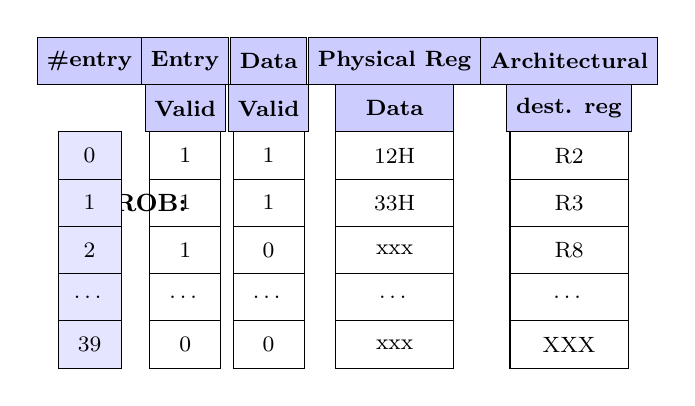
\begin{tikzpicture}
    \node[font=\small] at (-2.5,0) {\textbf{ROB:}};
    \matrix (rob) [matrix of nodes,
      nodes={draw, minimum width=1.2cm, minimum height=0.6cm, anchor=center, font=\footnotesize},
      row sep=-\pgflinewidth,
      column sep=-\pgflinewidth,
      column 1/.style={nodes={minimum width=0.8cm, fill=blue!10}},
      column 2/.style={nodes={minimum width=0.9cm}},
      column 3/.style={nodes={minimum width=0.9cm}},
      column 4/.style={nodes={minimum width=1.5cm}},
      column 5/.style={nodes={minimum width=1.5cm}},
      ampersand replacement=\&
      ] {
      |[fill=blue!20]| \textbf{\#entry} \& |[fill=blue!20]| \textbf{Entry} \& |[fill=blue!20]| \textbf{Data} \& |[fill=blue!20]| \textbf{Physical Reg} \& |[fill=blue!20]| \textbf{Architectural} \\
      \& |[fill=blue!20]| \textbf{Valid} \& |[fill=blue!20]| \textbf{Valid} \& |[fill=blue!20]| \textbf{Data} \& |[fill=blue!20]| \textbf{dest. reg} \\
      0 \& 1 \& 1 \& 12H \& R2 \\
      1 \& 1 \& 1 \& 33H \& R3 \\
      2 \& 1 \& 0 \& xxx \& R8 \\
      \dots \& \dots \& \dots \& \dots \& \dots \\
      39 \& 0 \& 0 \& xxx \& XXX \\
    };
  \end{tikzpicture}
\end{frame}

\begin{frame}{ARF -- Architectural Register File}
  \begin{itemize}
    \item \textbf{Holds the Architectural Register File}
    \begin{itemize}
      \item Architectural Registers are numbered: 0 -- R0, 1 -- R1, \dots
    \end{itemize}

    \vspace{0.3cm}

    \item \textbf{The value of an architectural register}
    \begin{itemize}
      \item is the value written to it by the last instruction committed which writes to this register
    \end{itemize}
  \end{itemize}

  \vspace{0.5cm}
  \centering
  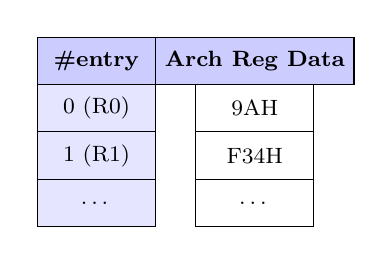
\begin{tikzpicture}
    \node[font=\small] at (-1.5,0) {\textbf{ARF:}};
    \matrix (arf) [matrix of nodes,
      nodes={draw, minimum width=1.5cm, minimum height=0.6cm, anchor=center, font=\footnotesize},
      row sep=-\pgflinewidth,
      column sep=-\pgflinewidth,
      column 1/.style={nodes={fill=blue!10}},
      ampersand replacement=\&
      ] {
      |[fill=blue!20]| \textbf{\#entry} \& |[fill=blue!20]| \textbf{Arch Reg Data} \\
      0 (R0) \& 9AH \\
      1 (R1) \& F34H \\
      \dots \& \dots \\
    };
  \end{tikzpicture}
\end{frame}

\begin{frame}{Reservation Station (RS)}
  \begin{itemize}
    \item \textbf{Pool of all ``not yet executed'' instructions}
    \begin{itemize}
      \item Holds the instruction's attributes and source data until it is executed
    \end{itemize}
  \end{itemize}

  \vspace{0.3cm}
  \centering
  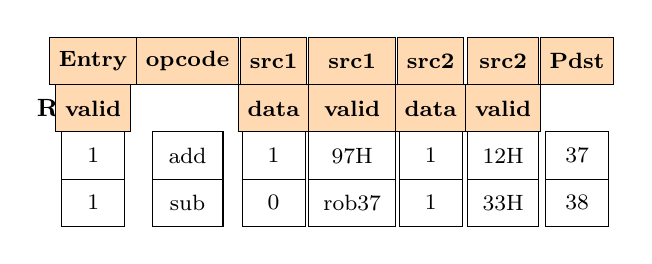
\begin{tikzpicture}
    \node[font=\small] at (-3.5,0.3) {\textbf{RS}};
    \matrix (rs) [matrix of nodes,
      nodes={draw, minimum width=1cm, minimum height=0.6cm, anchor=center, font=\footnotesize},
      row sep=-\pgflinewidth,
      column sep=-\pgflinewidth,
      column 1/.style={nodes={minimum width=0.8cm}},
      column 2/.style={nodes={minimum width=0.9cm}},
      column 3/.style={nodes={minimum width=0.8cm}},
      column 4/.style={nodes={minimum width=1.1cm}},
      column 5/.style={nodes={minimum width=0.8cm}},
      column 6/.style={nodes={minimum width=0.9cm}},
      column 7/.style={nodes={minimum width=0.8cm}},
      column 8/.style={nodes={minimum width=0.9cm}},
      ampersand replacement=\&
      ] {
      |[fill=orange!30]| \textbf{Entry} \& |[fill=orange!30]| \textbf{opcode} \& |[fill=orange!30]| \textbf{src1} \& |[fill=orange!30]| \textbf{src1} \& |[fill=orange!30]| \textbf{src2} \& |[fill=orange!30]| \textbf{src2} \& |[fill=orange!30]| \textbf{Pdst} \\
      |[fill=orange!30]| \textbf{valid} \& \& |[fill=orange!30]| \textbf{data} \& |[fill=orange!30]| \textbf{valid} \& |[fill=orange!30]| \textbf{data} \& |[fill=orange!30]| \textbf{valid} \& \\
      1 \& add \& 1 \& 97H \& 1 \& 12H \& 37 \\
      1 \& sub \& 0 \& rob37 \& 1 \& 33H \& 38 \\
    };
  \end{tikzpicture}

  \vspace{0.5cm}
  \begin{itemize}
    \item \textbf{When an instruction is allocated in RS, operand values are updated}
  \end{itemize}

  \vspace{0.2cm}
  \centering
  \begin{tabular}{|l|c|l|}
    \hline
    \textbf{Operand from} & \textbf{Data valid} & \textbf{Get value from} \\
    \hline
    architectural register & 1 & ARF \\
    \hline
    physical register & 1 & ROB \\
    \hline
    & 0 & Wait for value \\
    \hline
  \end{tabular}
\end{frame}

\begin{frame}{Reservation Station (RS) - Operation}
  \begin{itemize}
    \item \textbf{The RS maintains operands status ``ready/not-ready''}

    \vspace{0.3cm}

    \item Each cycle, executed instructions make more operands ``ready''
    \begin{itemize}
      \item The RS arbitrates the write-back busses between the execution units
      \item The RS monitors the write-back buses to capture data needed by awaiting instructions
      \item Data can be bypassed directly from a write-back bus to execution unit
    \end{itemize}

    \vspace{0.3cm}

    \item Instructions for which all operands are ready can be \emph{dispatched} for execution
    \begin{itemize}
      \item Dispatcher chooses which of the \emph{ready} instructions to execute next
      \item Dispatches chosen instructions to Execution Units
    \end{itemize}
  \end{itemize}

  \vspace{0.3cm}
  \centering
  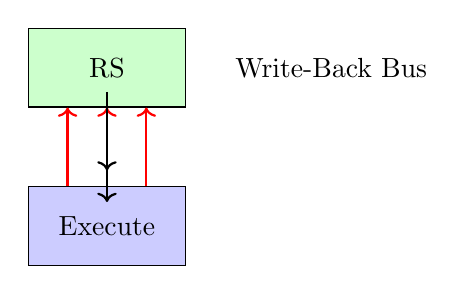
\begin{tikzpicture}
    \node[draw, fill=green!20, minimum width=2cm, minimum height=1cm] (rs) {RS};
    \node[draw, fill=blue!20, minimum width=2cm, minimum height=1cm, below=1cm of rs] (execute) {Execute};
    \draw[->, thick, red] ([xshift=-5mm]execute.north) -- ([xshift=-5mm]rs.south);
    \draw[->, thick, red] (execute.north) -- (rs.south);
    \draw[->, thick, red] ([xshift=5mm]execute.north) -- ([xshift=5mm]rs.south);
    \node[right=0.5cm of rs, align=left] {Write-Back Bus};
    \draw[->, thick] ([yshift=2mm]rs.south) -- ([yshift=2mm]execute.north);
    \draw[->, thick] ([yshift=-2mm]rs.south) -- ([yshift=-2mm]execute.north);
  \end{tikzpicture}
\end{frame}

\begin{frame}{Getting the Value of a Source Register}
  \textbf{Assume:} instruction X with architectural destination register Rj is allocated a physical register PRi (i.e., the instruction is allocated in ROB entry i)

  \vspace{0.3cm}

  \begin{itemize}
    \item \textbf{When instruction X finishes its execution}
    \begin{itemize}
      \item Write the result to PRi
      \item Match PRi against the physical sources of each instruction in the RS, and write the value of PRi to all matching sources in the RS
    \end{itemize}

    \vspace{0.2cm}

    \item \textbf{As long as no subsequent instruction has Rj as architectural destination register, and as long as instruction X does not retire, Rj remains mapped to PRi}
    \begin{itemize}
      \item For subsequent instructions allocated to the RS that have Rj as architectural source, their source is mapped to PRi, and they get the value of PRi from instruction X ROB entry
      \item This value is written as the source data in the RS upon allocation (and marked data valid)
    \end{itemize}

    \vspace{0.2cm}

    \item \textbf{When instruction X commits}
    \begin{itemize}
      \item Copy the value from the physical register, PRi, to the architectural register Rj in the ARF
      \item If the current mapping of the instruction's architectural destination register, Rj, is still the physical register allocated to the instruction, PRi:
      \begin{itemize}
        \item Set Rj's mapping to be architectural -- mapped to Rj in the ARF (Arch register file)
        \item As long as there is no subsequent instruction write to Rj, subsequent instructions that use Rj as source get the value of Rj from the ARF
      \end{itemize}
    \end{itemize}
  \end{itemize}
\end{frame}

\begin{frame}{Allocation and Renaming}
  \begin{itemize}
    \item \textbf{Perform register allocation and renaming for $\leq$4 instructions/cyc}

    \vspace{0.2cm}

    \item \textbf{The Register Alias Table maps architectural registers into physical registers}
    \begin{itemize}
      \item For each arch register, holds the number of latest physical register that updates it
      \item When a new instruction that writes to arch register R is allocated:
      \begin{itemize}
        \item Map R to the physical register which is used as the instruction destination
      \end{itemize}
    \end{itemize}

    \vspace{0.2cm}

    \item \textbf{The Allocator}
    \begin{itemize}
      \item Assigns to each instruction an entry number in the ROB / RS
      \item For each one of the sources (architectural registers) of the instruction:
      \begin{itemize}
        \item Lookup the Register Alias Table to find out the latest physical reg updating it
        \item Write it up in the RS entry
      \end{itemize}
    \end{itemize}
  \end{itemize}

  \vspace{0.3cm}
  \centering
  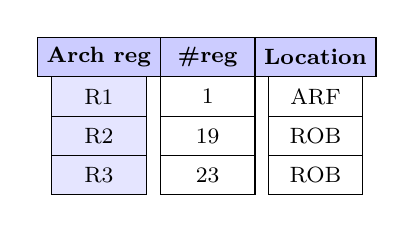
\begin{tikzpicture}
    \node[font=\small] at (-1.5,0) {\textbf{RAT:}};
    \matrix (rat) [matrix of nodes,
      nodes={draw, minimum width=1.2cm, minimum height=0.5cm, anchor=center, font=\footnotesize},
      row sep=-\pgflinewidth,
      column sep=-\pgflinewidth,
      column 1/.style={nodes={fill=blue!10}},
      ampersand replacement=\&
      ] {
      |[fill=blue!20]| \textbf{Arch reg} \& |[fill=blue!20]| \textbf{\#reg} \& |[fill=blue!20]| \textbf{Location} \\
      R1 \& 1 \& ARF \\
      R2 \& 19 \& ROB \\
      R3 \& 23 \& ROB \\
    };
  \end{tikzpicture}
\end{frame}

\begin{frame}{Register Renaming Example}
  \begin{tikzpicture}[font=\tiny, remember picture, overlay]
    % Explanation box in top left corner
    \node[draw, fill=yellow!10, inner sep=5pt, text width=5.5cm, align=left, anchor=north west] at ([xshift=0.2cm, yshift=-1.5cm]current page.north west) {
      \tiny
      \only<1>{
      \textbf{Step 1: First Instruction}\\[0.1cm]
      Instruction: \texttt{add R1$\leftarrow$R2,R1}\\[0.05cm]
      - Allocate ROB37 for R1\\
      - Update RAT: R1 maps to ROB37\\
      - Get sources from ARF(R1) and ROB19(R2)\\
      - Add entry to RS with both operands ready\\
      - ROB37 marked allocated but data invalid
      }
      \only<2>{
      \textbf{Step 2: After Execution}\\[0.1cm]
      - Instruction \texttt{add} completes execution\\
      - ROB37 data now valid (109H = 97H + 12H)\\
      - RS entry for \texttt{add} removed\\
      - Instruction ready to retire
      }
      \only<3>{
      \textbf{Step 3: Second Instruction}\\[0.1cm]
      Instruction: \texttt{sub R1$\leftarrow$R3,R1}\\[0.05cm]
      - Allocate ROB38 for R1\\
      - Update RAT: R1 now maps to ROB38\\
      - Get sources from ROB23(R3) and ROB37(R1)\\
      - RS entry waits for ROB37 (valid=0)\\
      - Shows WAW eliminated by renaming
      }
    };
  \end{tikzpicture}

  \centering
  \begin{tikzpicture}[font=\tiny]
    % IDQ at top
    \only<1>{
      \node[draw, fill=lightblue, inner sep=5pt] (idq) {\textbf{IDQ: add R1$\leftarrow$R2,R1}};
    }
    \only<2>{
      \node[draw, fill=green!30, inner sep=5pt] (idq) {\textbf{Executing add...}};
    }
    \only<3>{
      \node[draw, fill=lightblue, inner sep=5pt] (idq) {\textbf{IDQ: sub R1$\leftarrow$R3,R1}};
    }

    % RAT below IDQ
    \node[fill=green!10, inner sep=5pt, below=0.4cm of idq] (rat) {
      \begin{minipage}{4cm}
      \centering
      \textbf{RAT}

      \vspace{0.1cm}
      \tiny
      \only<1>{
      \begin{tabular}{|l|c|l|}
      \hline
      \textbf{Arch} & \textbf{Phys} & \textbf{Loc} \\
      \hline
      R1 & \textcolor{red}{37} & \textcolor{red}{ROB} \\
      \hdashline[2pt/2pt]
      R2 & 19 & ROB \\
      \hdashline[2pt/2pt]
      R3 & 23 & ROB \\
      \hline
      \end{tabular}
      }
      \only<2>{
      \begin{tabular}{|l|c|l|}
      \hline
      \textbf{Arch} & \textbf{Phys} & \textbf{Loc} \\
      \hline
      R1 & 37 & ROB \\
      \hdashline[2pt/2pt]
      R2 & 19 & ROB \\
      \hdashline[2pt/2pt]
      R3 & 23 & ROB \\
      \hline
      \end{tabular}
      }
      \only<3>{
      \begin{tabular}{|l|c|l|}
      \hline
      \textbf{Arch} & \textbf{Phys} & \textbf{Loc} \\
      \hline
      R1 & \textcolor{red}{38} & \textcolor{red}{ROB} \\
      \hdashline[2pt/2pt]
      R2 & 19 & ROB \\
      \hdashline[2pt/2pt]
      R3 & 23 & ROB \\
      \hline
      \end{tabular}
      }
      \end{minipage}
    };

    % ROB below and left of RAT
    \node[fill=cyan!10, inner sep=5pt, below=0.8cm of rat.south, anchor=north, xshift=-3.5cm] (rob) {
      \begin{minipage}{4.2cm}
      \centering
      \textbf{ROB}

      \vspace{0.1cm}
      \tiny
      \only<1>{
      \begin{tabular}{|c|c|c|c|}
      \hline
      \textbf{Phys} & \textbf{Alloc} & \textbf{Data} & \textbf{Arch} \\
      \textbf{Reg} & & \textbf{Valid} & \textbf{Reg} \\
      \hline
      19 & V & V & R2 \\
      \hdashline[2pt/2pt]
      23 & V & V & R3 \\
      \hdashline[2pt/2pt]
      \textcolor{red}{37} & \textcolor{red}{V} & \textcolor{red}{I} & \textcolor{red}{R1} \\
      \hdashline[2pt/2pt]
      38 & I & x & xxx \\
      \hline
      \end{tabular}
      }
      \only<2>{
      \begin{tabular}{|c|c|c|c|}
      \hline
      \textbf{Phys} & \textbf{Alloc} & \textbf{Data} & \textbf{Arch} \\
      \textbf{Reg} & & \textbf{Valid} & \textbf{Reg} \\
      \hline
      19 & V & V & R2 \\
      \hdashline[2pt/2pt]
      23 & V & V & R3 \\
      \hdashline[2pt/2pt]
      37 & V & \textcolor{blue!70!black}{V (109H)} & R1 \\
      \hdashline[2pt/2pt]
      38 & I & x & xxx \\
      \hline
      \end{tabular}
      }
      \only<3>{
      \begin{tabular}{|c|c|c|c|}
      \hline
      \textbf{Phys} & \textbf{Alloc} & \textbf{Data} & \textbf{Arch} \\
      \textbf{Reg} & & \textbf{Valid} & \textbf{Reg} \\
      \hline
      19 & V & V & R2 \\
      \hdashline[2pt/2pt]
      23 & V & V & R3 \\
      \hdashline[2pt/2pt]
      37 & V & V & R1 \\
      \hdashline[2pt/2pt]
      \textcolor{red}{38} & \textcolor{red}{V} & \textcolor{red}{I} & \textcolor{red}{R1} \\
      \hline
      \end{tabular}
      }
      \end{minipage}
    };

    % RS below and right of RAT
    \node[fill=orange!10, inner sep=5pt, below=0.8cm of rat.south, anchor=north, xshift=3.5cm] (rs) {
      \begin{minipage}{5cm}
      \centering
      \textbf{RS}

      \vspace{0.1cm}
      \tiny
      \only<1>{
      \begin{tabular}{|c|c|c|c|c|c|}
      \hline
      & \multicolumn{2}{c|}{\textbf{src1}} & \multicolumn{2}{c|}{\textbf{src2}} & \textbf{Pdst} \\
      \textbf{op} & \textbf{V} & \textbf{Val} & \textbf{V} & \textbf{Val} & \textbf{(ROB)} \\
      \hline
      \textcolor{red}{add} & \textcolor{red}{1} & \textcolor{red}{97H} & \textcolor{red}{1} & \textcolor{red}{12H} & \textcolor{red}{37} \\
      \hdashline[2pt/2pt]
      -- & -- & -- & -- & -- & -- \\
      \hline
      \end{tabular}
      }
      \only<2>{
      \begin{tabular}{|c|c|c|c|c|c|}
      \hline
      & \multicolumn{2}{c|}{\textbf{src1}} & \multicolumn{2}{c|}{\textbf{src2}} & \textbf{Pdst} \\
      \textbf{op} & \textbf{V} & \textbf{Val} & \textbf{V} & \textbf{Val} & \textbf{(ROB)} \\
      \hline
      -- & -- & -- & -- & -- & -- \\
      \hdashline[2pt/2pt]
      -- & -- & -- & -- & -- & -- \\
      \hline
      \end{tabular}
      }
      \only<3>{
      \begin{tabular}{|c|c|c|c|c|c|}
      \hline
      & \multicolumn{2}{c|}{\textbf{src1}} & \multicolumn{2}{c|}{\textbf{src2}} & \textbf{Pdst} \\
      \textbf{op} & \textbf{V} & \textbf{Val} & \textbf{V} & \textbf{Val} & \textbf{(ROB)} \\
      \hline
      -- & -- & -- & -- & -- & -- \\
      \hdashline[2pt/2pt]
      \textcolor{red}{sub} & \textcolor{red}{0} & \textcolor{red}{rob37} & \textcolor{red}{1} & \textcolor{red}{33H} & \textcolor{red}{38} \\
      \hline
      \end{tabular}
      }
      \end{minipage}
    };

    % ARF below ROB
    \node[fill=blue!15, inner sep=5pt, below=0.3cm of rob.south, anchor=north] (arf) {
      \begin{minipage}{2cm}
      \centering
      \tiny
      \textbf{ARF}

      \begin{tabular}{|c|c|}
      \hline
      R1 & 97H \\
      \hline
      \end{tabular}
      \end{minipage}
    };

    % Execute below RS
    \node[draw, fill=highlightorange, inner sep=5pt, below=0.5cm of rs.south east, anchor=east] (execute) {\textbf{Execute}};

    % Arrows
    \draw[->, thick] (idq.south) -- (rat.north);
    \draw[->, thick] (rat.south) -- ++(0,-0.3) -| (rob.north);
    \draw[->, thick] (rat.south) -- ++(0,-0.3) -| (rs.north);
    \draw[->, thick] (execute.north) -- (rs.south -| execute.north);
    \draw[->, thick] (execute.west) -| ([xshift=3mm]rob.east) -- (rob.east);

  \end{tikzpicture}
\end{frame}

\begin{frame}{Out-of-Order Core: Execution Units}
  \begin{center}
  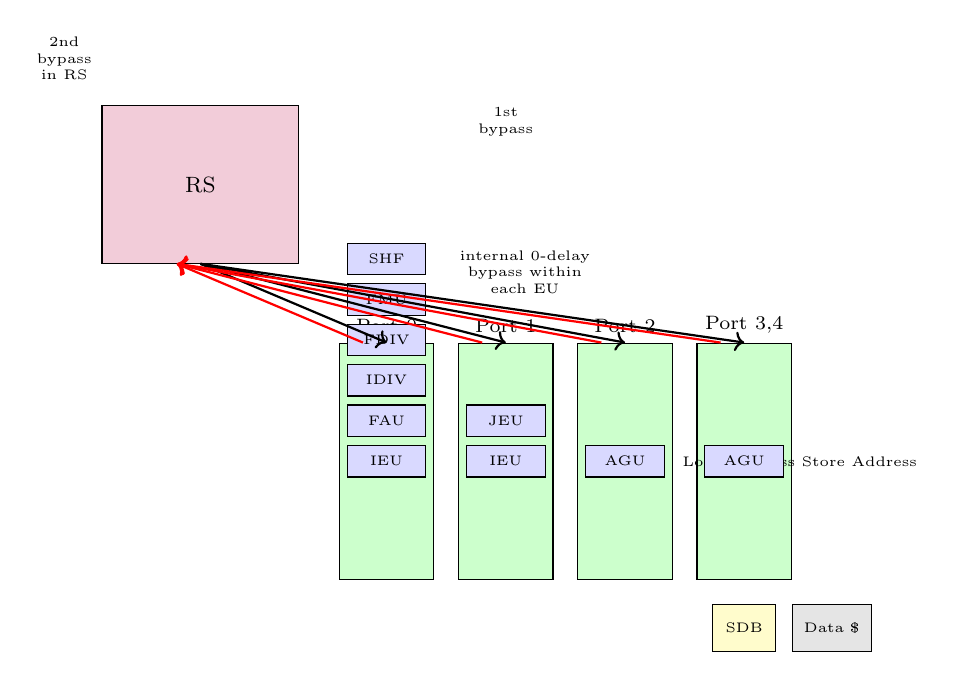
\begin{tikzpicture}[font=\footnotesize,
    port/.style={draw, fill=green!20, minimum width=1.2cm, minimum height=3cm},
    eu/.style={draw, fill=blue!15, minimum width=1cm, minimum height=0.4cm},
    ]

    % RS
    \node[draw, fill=purple!20, minimum width=2.5cm, minimum height=2cm] (rs) {RS};

    % Ports
    \node[port, below right=1cm and 0.5cm of rs] (port0) {};
    \node[above, font=\scriptsize] at (port0.north) {Port 0};

    \node[port, right=0.3cm of port0] (port1) {};
    \node[above, font=\scriptsize] at (port1.north) {Port 1};

    \node[port, right=0.3cm of port1] (port2) {};
    \node[above, font=\scriptsize] at (port2.north) {Port 2};

    \node[port, right=0.3cm of port2] (port34) {};
    \node[above, font=\scriptsize] at (port34.north) {Port 3,4};

    % Execution units in Port 0
    \node[eu] at (port0.center) (ieu0) {\tiny IEU};
    \node[eu, above=0.1cm of ieu0] (fau) {\tiny FAU};
    \node[eu, above=0.1cm of fau] (idiv) {\tiny IDIV};
    \node[eu, above=0.1cm of idiv] (fdiv) {\tiny FDIV};
    \node[eu, above=0.1cm of fdiv] (fmu) {\tiny FMU};
    \node[eu, above=0.1cm of fmu] (shf) {\tiny SHF};

    % Execution units in Port 1
    \node[eu] at (port1.center) (ieu1) {\tiny IEU};
    \node[eu, above=0.1cm of ieu1] (jeu) {\tiny JEU};

    % Execution units in Port 2
    \node[eu] at (port2.center) (agu2) {\tiny AGU};
    \node[right=0.1cm of agu2, font=\tiny] {Load Address};

    % Execution units in Port 3,4
    \node[eu] at (port34.center) (agu34) {\tiny AGU};
    \node[right=0.1cm of agu34, font=\tiny] {Store Address};

    % SDB and Data Cache
    \node[draw, fill=yellow!20, minimum width=0.8cm, minimum height=0.6cm, below=0.3cm of port34] (sdb) {\tiny SDB};
    \node[draw, fill=gray!20, minimum width=1cm, minimum height=0.6cm, right=0.2cm of sdb] (dcache) {\tiny Data \$};

    % Arrows from RS to ports
    \foreach \p in {port0, port1, port2, port34} {
      \draw[->, thick] (rs.south) -- (\p.north);
      \draw[<-, thick, red] ([xshift=-3mm]rs.south) -- ([xshift=-3mm]\p.north);
    }

    % Labels for bypass levels
    \node[above left=0.2cm and 0cm of rs, align=center, font=\tiny] {2nd\\bypass\\in RS};
    \node[above=2.5cm of port1, align=center, font=\tiny] {1st\\bypass};
    \node[above right=0.5cm and 0.2cm of port0, align=center, font=\tiny] {internal 0-delay\\bypass within\\each EU};
  \end{tikzpicture}
  \end{center}
\end{frame}

\begin{frame}{Execution Units Bypasses}
  \begin{center}
  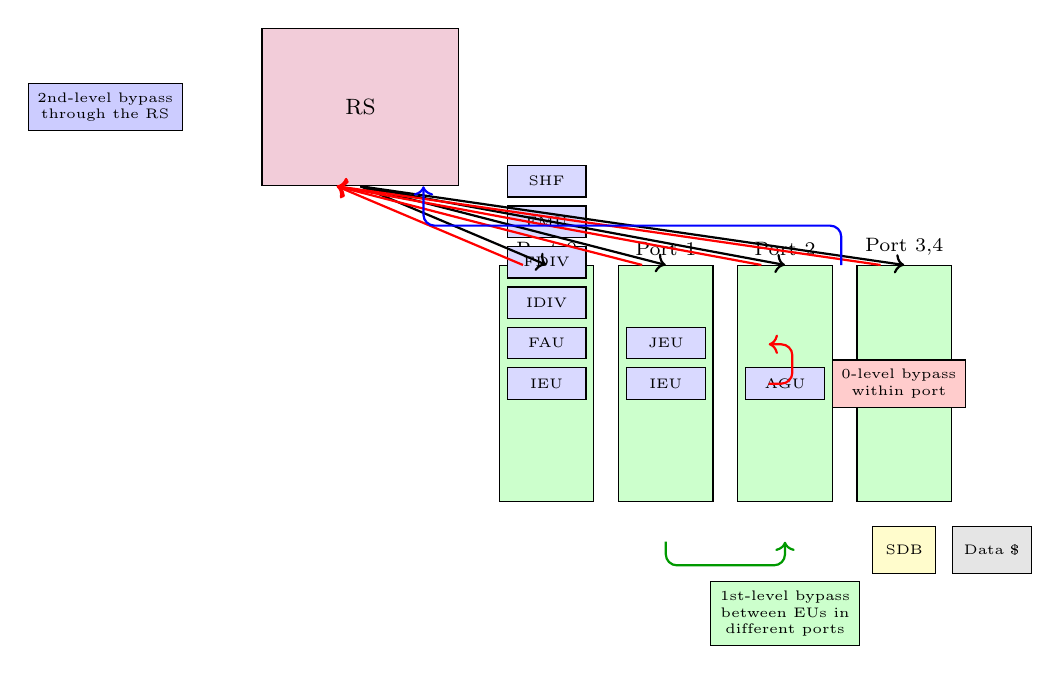
\begin{tikzpicture}[font=\footnotesize,
    port/.style={draw, fill=green!20, minimum width=1.2cm, minimum height=3cm},
    eu/.style={draw, fill=blue!15, minimum width=1cm, minimum height=0.4cm},
    ]

    % RS
    \node[draw, fill=purple!20, minimum width=2.5cm, minimum height=2cm] (rs) {RS};

    % Ports
    \node[port, below right=1cm and 0.5cm of rs] (port0) {};
    \node[above, font=\scriptsize] at (port0.north) {Port 0};

    \node[port, right=0.3cm of port0] (port1) {};
    \node[above, font=\scriptsize] at (port1.north) {Port 1};

    \node[port, right=0.3cm of port1] (port2) {};
    \node[above, font=\scriptsize] at (port2.north) {Port 2};

    \node[port, right=0.3cm of port2] (port34) {};
    \node[above, font=\scriptsize] at (port34.north) {Port 3,4};

    % Execution units in Port 0
    \node[eu] at (port0.center) (ieu0) {\tiny IEU};
    \node[eu, above=0.1cm of ieu0] (fau) {\tiny FAU};
    \node[eu, above=0.1cm of fau] (idiv) {\tiny IDIV};
    \node[eu, above=0.1cm of idiv] (fdiv) {\tiny FDIV};
    \node[eu, above=0.1cm of fdiv] (fmu) {\tiny FMU};
    \node[eu, above=0.1cm of fmu] (shf) {\tiny SHF};

    % Execution units in Port 1
    \node[eu] at (port1.center) (ieu1) {\tiny IEU};
    \node[eu, above=0.1cm of ieu1] (jeu) {\tiny JEU};

    % Execution units in Port 2
    \node[eu] at (port2.center) (agu2) {\tiny AGU};

    % Execution units in Port 3,4
    \node[eu] at (port34.center) (agu34) {\tiny AGU};

    % SDB and Data Cache
    \node[draw, fill=yellow!20, minimum width=0.8cm, minimum height=0.6cm, below=0.3cm of port34] (sdb) {\tiny SDB};
    \node[draw, fill=gray!20, minimum width=1cm, minimum height=0.6cm, right=0.2cm of sdb] (dcache) {\tiny Data \$};

    % Arrows from RS to ports
    \foreach \p in {port0, port1, port2, port34} {
      \draw[->, thick] (rs.south) -- (\p.north);
      \draw[<-, thick, red] ([xshift=-3mm]rs.south) -- ([xshift=-3mm]\p.north);
    }

    % Bypass illustrations
    % 0-level bypass within port (red loop on port 1)
    \draw[->, thick, red, rounded corners] ([xshift=8mm]ieu1.east) -- ++(0.3,0) -- ++(0,0.5) -- ++(-0.3,0);
    \node[draw, fill=red!20, align=center, font=\tiny, right=1.5cm of port1] (bypass0) {0-level bypass\\within port};

    % 1st-level bypass between ports (green from port 1 to port 2)
    \draw[->, thick, green!60!black, rounded corners] ([yshift=-5mm]port1.south) -- ++(0,-0.3) -| ([yshift=-5mm]port2.south);
    \node[draw, fill=green!20, align=center, font=\tiny, below=1cm of port2] (bypass1) {1st-level bypass\\between EUs in\\different ports};

    % 2nd-level bypass through RS (blue loop back to RS)
    \draw[->, thick, blue, rounded corners] ([xshift=-8mm]port34.north) -- ++(0,0.5) -| ([xshift=8mm]rs.south);
    \node[draw, fill=blue!20, align=center, font=\tiny, left=1cm of rs] (bypass2) {2nd-level bypass\\through the RS};
  \end{tikzpicture}
  \end{center}
\end{frame}

\begin{frame}{The Bypass Network}
  \begin{itemize}
    \item \textbf{Assume}
    \begin{itemize}
      \item Instruction Y assigned PR19 as its destination physical register; Y takes 1 cycle to execute
      \item Instruction X uses PR19 as a source, and its other source is an immediate value
      \item Back-to-back 0-level bypass at the same EU
      \item 3 cycle bypass 1-level bypass going to a different EU
    \end{itemize}

    \vspace{0.3cm}

    \item \textbf{The RS marks instruction X as ready in the following cases}
    \begin{itemize}
      \item Instruction Y finished execution before instruction X was allocated
      \begin{itemize}
        \item PR19 value is written to X's RS entry when X is allocated
        \item Instruction X is ready at allocation
      \end{itemize}
      \item Instruction Y is sent to the same EU that instruction X is assigned to
      \begin{itemize}
        \item Instruction X is marked ready, and sent to the EU in the next cycle
      \end{itemize}
      \item Instruction Y is sent to a different port than instruction X is assigned to
      \begin{itemize}
        \item Instruction X is marked ready 3 cycles later, and sent to the EU
      \end{itemize}
      \item Y is sent to execution before X is allocated, but still did not finish execution
      \begin{itemize}
        \item When Y finishes exe and its write-back value gets to the RS, X can use it
      \end{itemize}
    \end{itemize}
  \end{itemize}
\end{frame}

\begin{frame}{The Reorder Buffer (ROB)}
  \vspace{-0.5cm}
  \begin{columns}
    \begin{column}{0.65\textwidth}
      \begin{itemize}
        \item<1-> Instructions allocated in-order

        \item<2-> After instruction executes (OOO):
        \begin{itemize}
          \item Mark as \emph{executed} $\Rightarrow$ ready to retire
        \end{itemize}

        \item<3-> Retirement (in-order, oldest first):
        \begin{itemize}
          \item Only after all prior instructions retire
        \end{itemize}
        \item<3-> Upon retirement:
        \begin{itemize}
          \item Copy value from physical to architectural register
          \item Update ARF (Architectural Register File)
          \item Reclaim ROB entry
        \end{itemize}
      \end{itemize}
    \end{column}
    \begin{column}{0.35\textwidth}
      \begin{center}
        \begin{tikzpicture}[scale=0.8,
          rob entry/.style={draw, minimum width=2cm, minimum height=0.35cm, inner sep=0, anchor=north west},
          rob empty/.style={rob entry, fill=white},
          rob allocated/.style={rob entry, fill=green!30},
          rob new/.style={rob entry, fill=green!50},
          rob executed/.style={rob entry, fill=red!30},
          rob executed redder/.style={rob entry, fill=red!60},
          rob faulting/.style={rob entry, fill=red!30},
          rob handler/.style={rob entry, fill=purple!30}
        ]
          % Draw white background for all entries (all stages) with names
          \foreach \i in {-2,-1,0,...,16} {
            \node[rob empty] (entry\i) at (0,-\i*0.4+0.35) {};
          }

          % ROB label
          \node[above=0.1cm of entry-2.north, font=\small] {ROB};

          % Stage 1: All allocated (green)
          \only<1>{
            \foreach \i in {0,...,11} {
              \node[rob allocated] at (0,-\i*0.4+0.35) {};
            }
            % New entries (12, 13, 14) with special green
            \foreach \i in {12,13,14} {
              \node[rob new] at (0,-\i*0.4+0.35) {};
            }

            % Labels: retire points to first allocated, alloc points to first empty
            \node[left=0.5cm of entry0.west, anchor=east] (retire) {retire};
            \draw[->,thick] (retire) -- (entry0.west);
            \node[right=0.1cm of entry0.east, anchor=west] {oldest};

            % Faded previous state
            \node[left=0.5cm of entry12.west, anchor=east, opacity=0.4] (alloc_old) {alloc};
            \draw[->,thick, opacity=0.4] (alloc_old) -- (entry12.west);
            \node[right=0.1cm of entry11.east, anchor=west, opacity=0.4] (youngest_old) {youngest};

            % Current state
            \node[left=0.5cm of entry15.west, anchor=east] (alloc) {alloc};
            \draw[->,thick] (alloc) -- (entry15.west);
            \node[right=0.1cm of entry14.east, anchor=west] (youngest) {youngest};

            % "New entries" label inside the ROB
            \node[fill=green!50, inner sep=2pt, font=\tiny, align=center] at (entry13.center) {new\\entries};

            % Straight dashed arrow from old alloc to new alloc
            \draw[->,dashed,thick] (alloc_old.south) -- (alloc.north);

            % Straight dashed arrow from old youngest to new youngest
            \draw[->,dashed,thick] (youngest_old.south) -- (youngest.north);
          }

          % Stage 2: Some executed (same as stage 3 but not the top one)
          \only<2>{
            % Entry 0 is still allocated (green)
            \node[rob allocated] at (0,-0*0.4+0.35) {};
            % Executed entries (same pattern as stage 3, excluding entry 0)
            \foreach \i in {1,2,4,5,7,8,9} {
              \node[rob executed] at (0,-\i*0.4+0.35) {};
            }
            % Other allocated entries
            \foreach \i in {3,6,10,11,12,13,14} {
              \node[rob allocated] at (0,-\i*0.4+0.35) {};
            }

            % "Executed" labels inside the ROB for the three groups
            \node[fill=red!30, inner sep=2pt, font=\tiny] at ($(entry1)!0.5!(entry2)$) {executed};
            \node[fill=red!30, inner sep=2pt, font=\tiny] at ($(entry4)!0.5!(entry5)$) {executed};
            \node[fill=red!30, inner sep=2pt, font=\tiny] at (entry8.center) {executed};

            % Labels: retire points to first allocated, alloc points to first empty
            \node[left=0.5cm of entry0.west, anchor=east] (retire) {retire};
            \draw[->,thick] (retire) -- (entry0.west);
            \node[right=0.1cm of entry0.east, anchor=west] {oldest};
            \node[left=0.5cm of entry15.west, anchor=east] (alloc) {alloc};
            \draw[->,thick] (alloc) -- (entry15.west);
            \node[right=0.1cm of entry14.east, anchor=west] {youngest};
          }

          % Stage 3: Retirement - top three entries retired (faded)
          \only<3>{
            % Top entry is "redder" executed
            \node[rob executed redder] at (0,-0*0.4+0.35) {};
            % Entries 1 and 2 are executed
            \foreach \i in {1,2} {
              \node[rob executed] at (0,-\i*0.4+0.35) {};
            }
            % Other executed entries
            \foreach \i in {4,5,7,8,9} {
              \node[rob executed] at (0,-\i*0.4+0.35) {};
            }
            % Allocated entries
            \foreach \i in {3,6,10,11,12,13,14} {
              \node[rob allocated] at (0,-\i*0.4+0.35) {};
            }

            % Fade the top three entries (retired)
            \foreach \i in {0,1,2} {
              \node[rob entry, fill=white, opacity=0.4] at (0,-\i*0.4+0.35) {};
            }

            % "Reclaimed" label in the middle of the top three
            \node[fill=white, inner sep=2pt, font=\tiny, opacity=0.7] at (entry1.center) {reclaimed};

            % Faded previous state (old retire position)
            \node[left=0.5cm of entry0.west, anchor=east, opacity=0.4] (retire_old) {retire};
            \draw[->,thick, opacity=0.4] (retire_old) -- (entry0.west);
            \node[right=0.1cm of entry0.east, anchor=west, opacity=0.4] (oldest_old) {oldest};

            % Current state (new retire position at entry 3)
            \node[left=0.5cm of entry3.west, anchor=east] (retire) {retire};
            \draw[->,thick] (retire) -- (entry3.west);
            \node[right=0.1cm of entry3.east, anchor=west] (oldest) {oldest};

            % Dashed arrows from old positions to new positions
            \draw[->,dashed,thick] (retire_old.south) -- (retire.north);
            \draw[->,dashed,thick] (oldest_old.south) -- (oldest.north);

            % Alloc and youngest unchanged
            \node[left=0.5cm of entry15.west, anchor=east] (alloc) {alloc};
            \draw[->,thick] (alloc) -- (entry15.west);
            \node[right=0.1cm of entry14.east, anchor=west] {youngest};
          }
        \end{tikzpicture}
      \end{center}
    \end{column}
  \end{columns}
\end{frame}

\begin{frame}{Faults and Exceptions -- Architecture (Reminder)}
  \begin{itemize}
    \item \textbf{Exception}: Event during instruction execution (divide by 0, page fault, etc.)

    \item \textbf{Types}$^*$:
    \begin{itemize}
      \item \textbf{Fault}: Potentially recoverable $\Rightarrow$ return to faulting instruction
      \item \textbf{Trap}: Intentional (e.g., breakpoint) $\Rightarrow$ return to next instruction
      \item \textbf{Abort}: Unrecoverable $\Rightarrow$ terminate
    \end{itemize}

    \item \textbf{Handling}: CPU transfers control to handler, save/restore state

    \item \textbf{Priority \& Nesting}: Higher priority exceptions can interrupt handlers
  \end{itemize}

  \vfill
  {\tiny $^*$Non-Intel terminology (based on intent/recoverability)}
\end{frame}

\begin{frame}{Faults and Exceptions -- Microarchitecture}
  \vspace{-0.5cm}
  \begin{columns}
    \begin{column}{0.65\textwidth}
      \begin{itemize}
        \item \textbf{Faults/exceptions served in program order}
        \begin{itemize}
          \item<1-> At EXE: mark faulting instruction
          \begin{itemize}
            \item E.g., divide by 0, page fault
          \end{itemize}

          \item<2-> Instructions older than fault retire first

          \item<3-> Faulting instruction reaches retire $\Rightarrow$ handle fault

          \item<4-> Fault handling:
          \begin{itemize}
            \item Flush ROB and pipeline
            \item Transfer control to fault handler
          \end{itemize}
        \end{itemize}
      \end{itemize}
    \end{column}
    \begin{column}{0.35\textwidth}
      \begin{center}
        \begin{tikzpicture}[scale=0.8,
          rob entry/.style={draw, minimum width=2cm, minimum height=0.35cm, inner sep=0, anchor=north west},
          rob empty/.style={rob entry, fill=white},
          rob allocated/.style={rob entry, fill=green!30},
          rob executed/.style={rob entry, fill=red!30},
          rob executed redder/.style={rob entry, fill=red!60},
          rob faulting/.style={rob entry, fill=orange!60},
          rob handler/.style={rob entry, fill=purple!30}
        ]
          % Draw white background for all entries (all stages) with names
          \foreach \i in {-2,-1,0,...,16} {
            \node[rob empty] (entry\i) at (0,-\i*0.4+0.35) {};
          }

          % ROB label
          \node[above=0.1cm of entry-2.north, font=\small] {ROB};

          % Stage 1: ROB state with faulting instruction (top 3 retired/empty)
          \only<1>{
            % Top 3 entries are empty (already white from background)
            % Entry 3 is allocated
            \node[rob allocated] at (0,-3*0.4+0.35) {};
            % Faulting instruction at entry 4
            \node[rob faulting] at (0,-4*0.4+0.35) {};
            % Other executed entries
            \foreach \i in {5,7,8,9} {
              \node[rob executed] at (0,-\i*0.4+0.35) {};
            }
            % Other allocated entries
            \foreach \i in {6,10,11,12,13,14} {
              \node[rob allocated] at (0,-\i*0.4+0.35) {};
            }

            % "Exception" label on the faulting instruction
            \node[inner sep=0pt, font=\tiny] at (entry4.center) {exception};

            % Labels: retire points to entry 3
            \node[left=0.5cm of entry3.west, anchor=east] (retire) {retire};
            \draw[->,thick] (retire) -- (entry3.west);
            \node[right=0.1cm of entry3.east, anchor=west] {oldest};
            \node[left=0.5cm of entry15.west, anchor=east] (alloc) {alloc};
            \draw[->,thick] (alloc) -- (entry15.west);
            \node[right=0.1cm of entry14.east, anchor=west] {youngest};
          }

          % Stage 2: Entry 3 retired (older than fault)
          \only<2>{
            % Entry 3 is now redder (retired/committed)
            \node[rob executed redder] at (0,-3*0.4+0.35) {};
            % Faulting instruction at entry 4
            \node[rob faulting] at (0,-4*0.4+0.35) {};
            % Other executed entries
            \foreach \i in {5,7,8,9} {
              \node[rob executed] at (0,-\i*0.4+0.35) {};
            }
            % Other allocated entries
            \foreach \i in {6,10,11,12,13,14} {
              \node[rob allocated] at (0,-\i*0.4+0.35) {};
            }

            % "Exception" label on the faulting instruction
            \node[inner sep=0pt, font=\tiny] at (entry4.center) {exception};

            % Labels: retire still at entry 3 (but now retired)
            \node[left=0.5cm of entry3.west, anchor=east] (retire) {retire};
            \draw[->,thick] (retire) -- (entry3.west);
            \node[right=0.1cm of entry3.east, anchor=west] {oldest};
            \node[left=0.5cm of entry15.west, anchor=east] (alloc) {alloc};
            \draw[->,thick] (alloc) -- (entry15.west);
            \node[right=0.1cm of entry14.east, anchor=west] {youngest};
          }

          % Stage 3: Entry 3 retired, faulting instruction now at retire
          \only<3>{
            % Entry 3 is regular red (executed)
            \node[rob executed] at (0,-3*0.4+0.35) {};
            % Faulting instruction at entry 4
            \node[rob faulting] at (0,-4*0.4+0.35) {};
            % Other executed entries
            \foreach \i in {5,7,8,9} {
              \node[rob executed] at (0,-\i*0.4+0.35) {};
            }
            % Other allocated entries
            \foreach \i in {6,10,11,12,13,14} {
              \node[rob allocated] at (0,-\i*0.4+0.35) {};
            }

            % Fade entry 3 (retired)
            \node[rob entry, fill=white, opacity=0.4] at (0,-3*0.4+0.35) {};

            % "Retired" label on entry 3
            \node[fill=white, inner sep=0pt, font=\tiny, opacity=0.7] at (entry3.center) {retired};

            % "Exception" label on the faulting instruction
            \node[inner sep=0pt, font=\tiny] at (entry4.center) {exception};

            % Faded previous state (old retire position at entry 3)
            \node[left=0.5cm of entry3.west, anchor=east, opacity=0.4] (retire_old) {retire};
            \draw[->,thick, opacity=0.4] (retire_old) -- (entry3.west);
            \node[right=0.1cm of entry3.east, anchor=west, opacity=0.4] (oldest_old) {oldest};

            % Current state (new retire position at entry 4 - the faulting instruction)
            \node[left=0.5cm of entry4.west, anchor=east] (retire) {retire};
            \draw[->,thick] (retire) -- (entry4.west);
            \node[right=0.1cm of entry4.east, anchor=west] (oldest) {oldest};

            % Curved dashed arrows from old positions to new positions
            \draw[->,dashed,thick] (retire_old.west) to[out=180,in=180] (retire.west);
            \draw[->,dashed,thick] (oldest_old.east) to[out=0,in=0] (oldest.east);

            % Alloc and youngest unchanged
            \node[left=0.5cm of entry15.west, anchor=east] (alloc) {alloc};
            \draw[->,thick] (alloc) -- (entry15.west);
            \node[right=0.1cm of entry14.east, anchor=west] {youngest};
          }

          % Stage 4: Flush begins - entries faded, alloc moves to faulting instruction
          \only<4>{
            % Entry 3 is empty (retired, not shown)
            % Faulting instruction at entry 4
            \node[rob faulting] at (0,-4*0.4+0.35) {};
            % Other executed entries
            \foreach \i in {5,7,8,9} {
              \node[rob executed] at (0,-\i*0.4+0.35) {};
            }
            % Other allocated entries
            \foreach \i in {6,10,11,12,13,14} {
              \node[rob allocated] at (0,-\i*0.4+0.35) {};
            }

            % Fade all entries (being flushed)
            \foreach \i in {4,5,6,7,8,9,10,11,12,13,14} {
              \node[rob entry, fill=white, opacity=0.5] at (0,-\i*0.4+0.35) {};
            }

            % "Exception" label on the faulting instruction (faded)
            \node[inner sep=0pt, font=\tiny, opacity=0.5] at (entry4.center) {exception};

            % "Flushed" label rotated 45 degrees in the middle of flushed entries
            \node[rotate=45, font=\small, opacity=0.6] at (entry9.center) {flushed};

            % retire stays at entry 4
            \node[left=0.5cm of entry4.west, anchor=east] (retire) {retire};
            \draw[->,thick] (retire) -- (entry4.west);
            \node[right=0.1cm of entry4.east, anchor=west] (oldest) {oldest};

            % Faded old alloc at entry 15
            \node[left=0.5cm of entry15.west, anchor=east, opacity=0.4] (alloc_old) {alloc};
            \draw[->,thick, opacity=0.4] (alloc_old) -- (entry15.west);
            \node[right=0.1cm of entry14.east, anchor=west, opacity=0.4] (youngest_old) {youngest};

            % New alloc at entry 4 (same as retire)
            \node[left=0.5cm of entry4.west, anchor=east, yshift=-0.5cm] (alloc) {alloc};
            \draw[->,thick] (alloc) -- (entry4.west);

            % Dashed arrow from old alloc to new alloc
            \draw[->,dashed,thick] (alloc_old.north) -- (alloc.south);
          }
        \end{tikzpicture}
      \end{center}
    \end{column}
  \end{columns}
\end{frame}

\begin{frame}{Interrupts -- Architecture (Reminder)}
  \begin{itemize}
    \item \textbf{Purpose}: Handle asynchronous external events (I/O, timers, etc.)

    \item \textbf{Key characteristics}:
    \begin{itemize}
      \item \textbf{Asynchronous}: Not tied to any instruction
      \item Transfer control to handler, save/restore state (similar to exceptions)
      \item Return to next instruction
    \end{itemize}

    \item \textbf{Interrupt masking}:
    \begin{itemize}
      \item Can be masked/enabled via processor flags
      \item CPU automatically masks interrupts during handler entry
    \end{itemize}
  \end{itemize}
\end{frame}

\begin{frame}{Interrupts}
  \begin{columns}
    \begin{column}{0.65\textwidth}
      \begin{itemize}
        \item \textbf{Interrupts served when next instruction retires}
        \begin{itemize}
          \item Let current cycle instruction retire
        \end{itemize}
      \end{itemize}
    \end{column}
    \begin{column}{0.35\textwidth}
      \begin{center}
        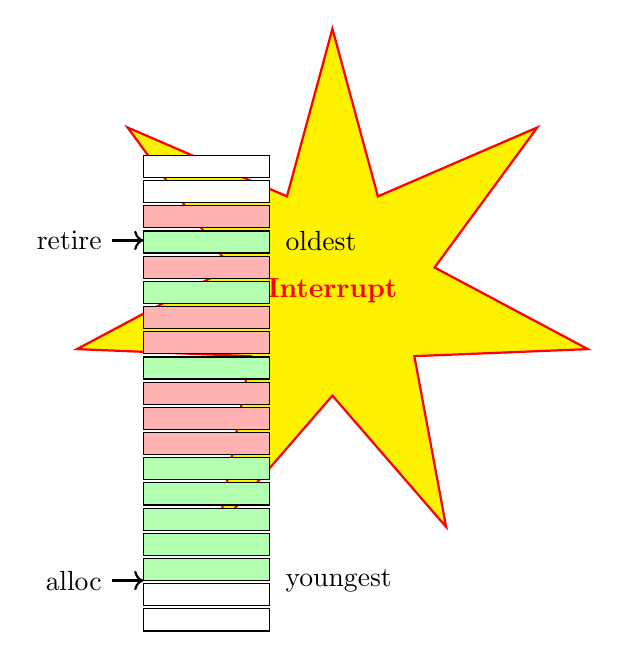
\begin{tikzpicture}[scale=0.8]
          % Interrupt indicator
          \node[star, star points=7, star point ratio=2.5, draw=red, thick, fill=yellow, minimum size=1.5cm] at (3,-1) {\textcolor{red}{\textbf{Interrupt}}};

          % ROB visualization
          \foreach \i in {0,2,4,5,7,8,9} {
            \draw[fill=red!30] (0,-\i*0.4) rectangle (2,-\i*0.4+0.35);
          }
          \foreach \i in {1,3,6,10,11,12,13,14} {
            \draw[fill=green!30] (0,-\i*0.4) rectangle (2,-\i*0.4+0.35);
          }

          % Empty entries
          \foreach \i in {-2,-1,15,16} {
            \draw[fill=white] (0,-\i*0.4) rectangle (2,-\i*0.4+0.35);
          }

          % Labels
          \draw[->,thick] (-0.5,-0.2) -- (0,-0.2) node[left] at (-0.5,-0.2) {retire};
          \node[right] at (2.1,-0.2) {oldest};

          \draw[->,thick] (-0.5,-5.6) -- (0,-5.6) node[left] at (-0.5,-5.6) {alloc};
          \node[right] at (2.1,-5.6) {youngest};
        \end{tikzpicture}
      \end{center}
    \end{column}
  \end{columns}
\end{frame}

\begin{frame}{Interrupts}
  \begin{columns}
    \begin{column}{0.65\textwidth}
      \begin{itemize}
        \item \textbf{Interrupts served when next instruction retires}
        \begin{itemize}
          \item Let current cycle instruction retire
          \item Flush subsequent instructions
        \end{itemize}
      \end{itemize}
    \end{column}
    \begin{column}{0.35\textwidth}
      \begin{center}
        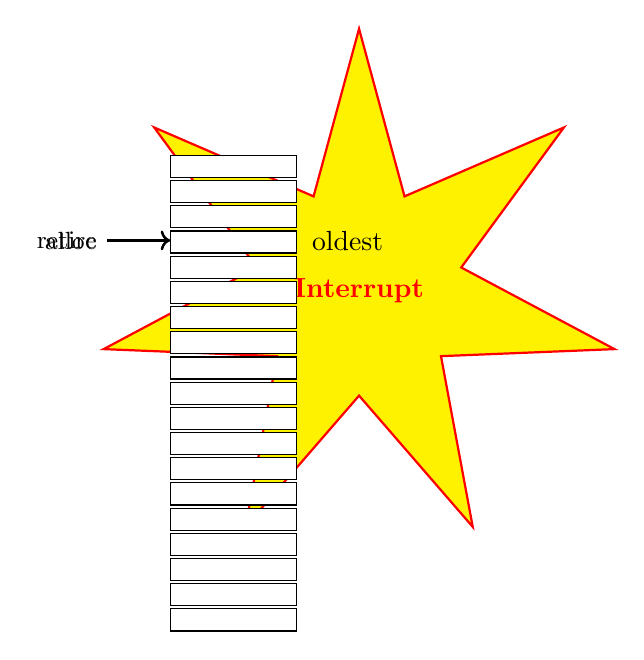
\begin{tikzpicture}[scale=0.8]
          % Interrupt indicator
          \node[star, star points=7, star point ratio=2.5, draw=red, thick, fill=yellow, minimum size=1.5cm] at (3,-1) {\textcolor{red}{\textbf{Interrupt}}};

          % Empty ROB after flush
          \foreach \i in {-2,-1,0,...,16} {
            \draw[fill=white] (0,-\i*0.4) rectangle (2,-\i*0.4+0.35);
          }

          % Labels
          \draw[->,thick] (-1,-0.2) -- (0,-0.2) node[left] at (-1,-0.2) {\small retire};
          \node[right] at (2.1,-0.2) {oldest};

          \draw[->,thick] (-1,-0.2) -- (0,-0.2) node[left] at (-1,-0.2) {\small alloc};
        \end{tikzpicture}
      \end{center}
    \end{column}
  \end{columns}
\end{frame}

\begin{frame}{Interrupts}
  \begin{columns}
    \begin{column}{0.65\textwidth}
      \begin{itemize}
        \item \textbf{Interrupts served when next instruction retires}
        \begin{itemize}
          \item Let current cycle instruction retire
          \item Flush subsequent instructions
          \item Initiate interrupt service code
          \item Re-fetch subsequent instructions
        \end{itemize}
      \end{itemize}
    \end{column}
    \begin{column}{0.35\textwidth}
      \begin{center}
        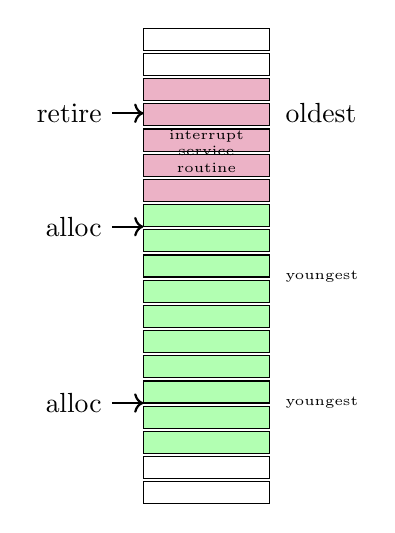
\begin{tikzpicture}[scale=0.8]
          % Interrupt service routine
          \foreach \i in {0,1,2,3,4} {
            \draw[fill=purple!30] (0,-\i*0.4) rectangle (2,-\i*0.4+0.35);
          }
          \node[font=\tiny,align=center] at (1,-0.8) {interrupt\\service\\routine};

          % Re-fetched instructions
          \foreach \i in {5,...,9} {
            \draw[fill=green!30] (0,-\i*0.4) rectangle (2,-\i*0.4+0.35);
          }
          \node[right,font=\tiny] at (2.1,-7*0.4) {youngest};

          \foreach \i in {10,...,14} {
            \draw[fill=green!30] (0,-\i*0.4) rectangle (2,-\i*0.4+0.35);
          }
          \node[right,font=\tiny] at (2.1,-12*0.4) {youngest};

          % Empty entries
          \foreach \i in {-2,-1,15,16} {
            \draw[fill=white] (0,-\i*0.4) rectangle (2,-\i*0.4+0.35);
          }

          % Labels
          \draw[->,thick] (-0.5,-0.2) -- (0,-0.2) node[left] at (-0.5,-0.2) {retire};
          \node[right] at (2.1,-0.2) {oldest};

          \draw[->,thick] (-0.5,-2.0) -- (0,-2.0) node[left] at (-0.5,-2.0) {alloc};

          \draw[->,thick] (-0.5,-4.8) -- (0,-4.8) node[left] at (-0.5,-4.8) {alloc};
        \end{tikzpicture}
      \end{center}
    \end{column}
  \end{columns}
\end{frame}

\begin{frame}{Large ROB and RS are Important}
  \begin{itemize}
    \item \textbf{A Large RS}
    \begin{itemize}
      \item Increases the window in which we look for independent instructions
      \item Exposes more parallelism potential
    \end{itemize}

    \vspace{0.5cm}

    \item \textbf{Large ROB}
    \begin{itemize}
      \item The ROB is a superset of the RS $\Rightarrow$ ROB size $\geq$ RS size
      \item Allows covering long latency operations (cache miss, divide)
    \end{itemize}
  \end{itemize}
\end{frame}

\begin{frame}{Large ROB and RS -- Example}
  \textbf{Scenario:} A Load misses the L1 cache and hits the L2 cache

  \vspace{0.1cm}

  \begin{itemize}
    \item Data takes $\sim$10 cycles to return
    \begin{itemize}
      \item With 3 instructions fetched per cycle $\Rightarrow$ $\sim$30 new instructions get into pipeline during this time
    \end{itemize}

    \vspace{0.3cm}

    \item Instructions following the Load cannot commit
    \begin{itemize}
      \item $\Rightarrow$ They pile up in the ROB
    \end{itemize}

    \vspace{0.3cm}

    \item Instructions \emph{independent} of the Load are executed and leave the RS
    \begin{itemize}
      \item As long as the ROB is not full, we can keep fetching, renaming, and executing instructions
    \end{itemize}
  \end{itemize}

  \vspace{0.3cm}

  \begin{alertblock}{Key Point}
    Large ROB and RS allow the processor to continue making progress despite long-latency operations
  \end{alertblock}
\end{frame}

\begin{frame}{Out Of Order Execution Summary}
  \begin{itemize}
    \item \textbf{Core Concept}
    \begin{itemize}
      \item Look ahead in a window of instructions
      \item Dispatch \emph{ready instructions} to execution:
      \begin{itemize}
        \item All source data is available (no dependencies on pending instructions)
        \item Required execution resources are available
      \end{itemize}
    \end{itemize}

    \vspace{0.3cm}

    \item \textbf{Key Advantages}
    \begin{itemize}
      \item Exploit Instruction Level Parallelism (ILP) beyond adjacent instructions
      \item Hide long latencies (e.g., L1 cache miss, divide operations)
      \item Complements and surpasses compile-time scheduling:
      \begin{itemize}
        \item Can exploit ILP across conditional branches (using speculation)
        \item Adapts to actual execution behavior at runtime
        \item Register renaming enables use of more than architectural registers
      \end{itemize}
    \end{itemize}

    \vspace{0.3cm}

    \item \textbf{Implementation Cost}
    \begin{itemize}
      \item Complex micro-architecture: register renaming, scheduler, recovery logic
      \item Memory ordering challenges (coming next)
    \end{itemize}
  \end{itemize}
\end{frame}

\begin{frame}
  \begin{center}
    \vspace{3cm}
    {\Huge \textbf{OOO Execution of Memory Operations}}
  \end{center}
\end{frame}

\begin{frame}{OOO Execution of Memory Operations}
  \begin{itemize}
    \item \textbf{The RS dispatches instructions based on \textcolor{green}{register} dependencies}
    \begin{itemize}
      \item The RS cannot detect \textcolor{purple}{memory} dependencies
      \begin{center}
        \texttt{store Mem[r1+r3*2] $\leftarrow$ r9}\\
        \texttt{load  r2 $\leftarrow$ Mem[r10+r7*2]}
      \end{center}
      \begin{itemize}
        \item Does not know the load/store memory addresses
      \end{itemize}
      
      \item The RS dispatches load/store instructions to the Address Generation Unit (AGU) when the sources for the address calculation are ready
      
      \item The AGU calculates the virtual memory address:
      \begin{center}
        \colorbox{gray!20}{Base Register + (Scale × Index Register) + Displacement}
      \end{center}
    \end{itemize}
    
    \item \textbf{The AGU sends the address to the Memory Order Buffer (MOB)}
    \begin{itemize}
      \item The MOB resolves memory dependencies and enforces memory ordering
    \end{itemize}
  \end{itemize}
\end{frame}

\begin{frame}{Load/Store Ordering}
  \begin{itemize}
    \item \textbf{Loads can be executed OOO with respect to other loads}
    \begin{itemize}
      \item Not allowing this would have a very big performance impact
    \end{itemize}
    
    \item \textbf{Stores write value to the data-cache in-order, post retirement}
    \begin{itemize}
      \item Stores cannot write values to the data-cache speculatively
      \begin{itemize}
        \item There is no simple way to undo them
      \end{itemize}
      \item Stores to the data-cache are never re-ordered among themselves
      \begin{itemize}
        \item Must be seen in-order to other cores or agents
      \end{itemize}
    \end{itemize}
    
    \item \textbf{Loads need to maintain correct order with respect to stores}
    \begin{itemize}
      \item The RS dispatches instructions based on \textcolor{gray}{register dependencies}
      \begin{itemize}
        \item The RS cannot detect memory dependencies
      \end{itemize}
      \item The MOB tracks dependencies between loads and stores
    \end{itemize}
  \end{itemize}
\end{frame}

\begin{frame}{Load/Store Ordering}
    The MOB tracks dependencies between loads and stores
    \begin{block}{An older Store has an unresolved address $\rightarrow$ block Load}
      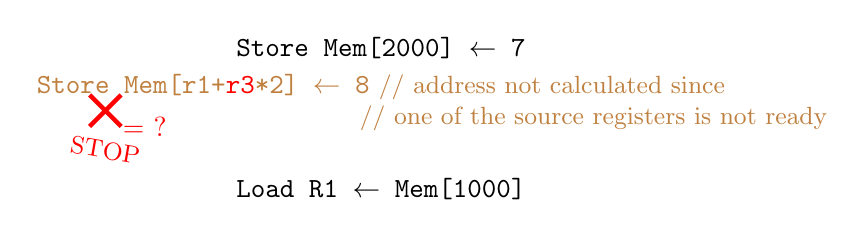
\begin{tikzpicture}[remember picture]
        \node[align=left] at (4,1.5) {\texttt{Store Mem[2000] $\leftarrow$ 7}};
        \node[align=left, brown] at (4,1) {\texttt{Store Mem[r1+\tikzmark{r3}\textcolor{red}{r3}*2] $\leftarrow$ 8} \small // address not calculated since};
        \node[align=left, brown] at (6.7,0.6) {\small // one of the source registers is not ready};
        \node[red] at (1,0.5) {= ?};
        \draw[red, ultra thick] (0.3,0.5) -- (0.7,0.9);
        \draw[red, ultra thick] (0.3,0.9) -- (0.7,0.5);
        \node[red, rotate=-10] at (0.5,0.2) {\small STOP};
        \node[align=left] at (4,-0.3) {\texttt{Load R1 $\leftarrow$ Mem[\tikzmark{target}1000]}};
      \end{tikzpicture}
      \begin{tikzpicture}[remember picture, overlay]
        \draw[->, red, thick] ([xshift=4pt,yshift=-1pt]pic cs:r3) -- ([xshift=5,yshift=12pt]pic cs:target);
      \end{tikzpicture}
    \end{block}
    \begin{block}{Older Store to same address, but Store's data \underline{is not ready} $\rightarrow$ block Load}
    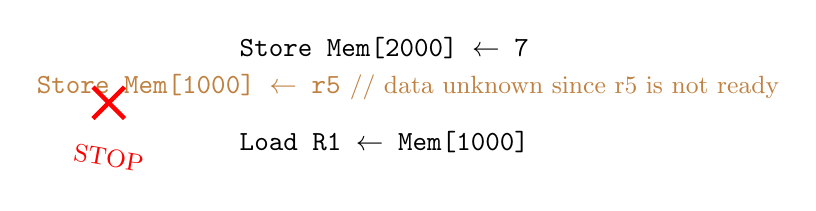
\begin{tikzpicture}
      \node[align=left] at (4,1.2) {\texttt{Store Mem[2000] $\leftarrow$ 7}};
      \node[align=left, brown] at (4.3,0.7) {\texttt{Store Mem[1000] $\leftarrow$ r5} \small // data unknown since r5 is not ready};
      \draw[red, ultra thick] (0.3,0.3) -- (0.7,0.7);
      \draw[red, ultra thick] (0.3,0.7) -- (0.7,0.3);
      \node[red, rotate=-10] at (0.5,-0.2) {\small STOP};
      \node[align=left] at (4,0) {\texttt{Load R1 $\leftarrow$ Mem[1000]}};
    \end{tikzpicture}
    \end{block}
\end{frame}

\begin{frame}{Store Implemented as 2 $\mu$ops}
  \begin{itemize}
    \item \textbf{Stores are decoded into two independent $\mu$ops}
    \begin{itemize}
      \item STA (store-address): calculates the address of the store
      \item STD (store-data): stores the data into the Store Data buffer
      \begin{itemize}
        \item This makes the data available to any Load that needs it
        \item The actual write to memory is done when the store retires
      \end{itemize}
    \end{itemize}
    
    \vspace{0.5cm}
    
    \item \textbf{Separating Store to STA \& STD improves performance}
    \begin{itemize}
      \item Allows STA to dispatch earlier, even before the data is known
      \begin{itemize}
        \item Address conflicts resolved earlier $\Rightarrow$\\
        opens memory pipeline for other loads
      \end{itemize}
      
      \item STA and STD can be issued to execution units in parallel
      \begin{itemize}
        \item STA dispatched to AGU when its sources (base + index) are ready
        \item STD dispatched to SDB when its source operand is available
      \end{itemize}
    \end{itemize}
  \end{itemize}
\end{frame}


\begin{frame}{Memory Order Buffer (MOB)}
  \begin{columns}
    \begin{column}{0.7\textwidth}
      \begin{itemize}
        \item \textbf{Store Coloring}
        \begin{itemize}
          \item Stores: track in \emph{Store Buffer} $\rightarrow$ alloc \textbf{SBID}
          \item Loads: track in \emph{Load Buffer} $\rightarrow$ alloc \textbf{LBID}, save \textbf{SBID}
          \item In-order allocation
        \end{itemize}
        
        \item \textbf{Loads check against prior stores}
        \begin{itemize}
          \item Those with SBID $\leq$ load's SBID
        \end{itemize}
        
        \item \textbf{Load blocks when:}
        \begin{itemize}
          \item Relevant STA has unresolved address
          \item STA to same address awaits data
          \item Data cache misses
        \end{itemize}
        
        \item \textbf{MOB handles blocked loads:}
        \begin{itemize}
          \item Records blocking info in Load Buffer
          \item Re-dispatches on wake-up signal
          \item May block again on new condition
        \end{itemize}
        
        \item \textbf{Unblocked loads → execute (bypass)}
      \end{itemize}
    \end{column}
    
    \begin{column}{0.3\textwidth}
      \begin{center}
        \begin{tabular}{|c|c|c|}
          \hline
          & \textbf{LBID} & \textbf{SBID} \\
          \hline
          \rowcolor{blue!15} Store & - & 0 \\
          \hline
          \rowcolor{green!15} Store & - & 1 \\
          \hline
          \rowcolor{green!15} Load & 0 & 1 \\
          \hline
          \rowcolor{orange!15} Store & - & 2 \\
          \hline
          \rowcolor{orange!15} Load & 1 & 2 \\
          \hline
          \rowcolor{orange!15} Load & 2 & 2 \\
          \hline
          \rowcolor{orange!15} Load & 3 & 2 \\
          \hline
          \rowcolor{red!15} Store & - & 3 \\
          \hline
          \rowcolor{red!15} Load & 4 & 3 \\
          \hline
        \end{tabular}
      \end{center}
    \end{column}
  \end{columns}
\end{frame}


% Updated macro with more flexibility and queue colors
\newcommand{\drawpipelineCustomExt}[9]{%
    % Parameters: 
    % #1: Predict/Fetch color (0=normal, 1=highlight, 2=gray)
    % #2: Decode color
    % #3: Alloc color  
    % #4: Schedule/EX color
    % #5: Retire color
    % #6: IQ queue color (0=green, 1=gray, 2=half gray/half green)
    % #7: uopq queue color (0=green, 1=gray, 2=half gray/half green)
    % #8: RS queue color (0=green, 1=gray, 2=half gray/half green)
    % #9: ROB queue color (0=green, 1=gray, 2=half gray/half green)
    \begin{tikzpicture}[
        remember picture,
        stage/.style={rectangle, draw=black, thick, minimum width=2.2cm, minimum height=0.9cm, font=\footnotesize, fill=orange!40},
        stageHighlight/.style={stage, fill=yellow!60},
        stageGray/.style={stage, fill=gray!30},
        queue/.style={rectangle, draw=black, fill=green!60, minimum width=0.15cm, minimum height=0.7cm},
        queueGray/.style={rectangle, draw=black, fill=gray!30, minimum width=0.15cm, minimum height=0.7cm},
        scale=0.75, transform shape
    ]
        
        % Predict/Fetch
        \ifnum#1=1
            \node[stageHighlight] (fetch) {Predict/Fetch};
        \else
            \ifnum#1=2
                \node[stageGray] (fetch) {Predict/Fetch};
            \else
                \node[stage] (fetch) {Predict/Fetch};
            \fi
        \fi
        
        % IQ queue
        \ifnum#6=1
            \node[queueGray, right=0.1cm of fetch] (iq1) {};
            \node[queueGray, right=0 of iq1] (iq2) {};
            \node[queueGray, right=0 of iq2] (iq3) {};
            \node[queueGray, right=0 of iq3] (iq4) {};
        \else
            \ifnum#6=2
                \node[queueGray, right=0.1cm of fetch] (iq1) {};
                \node[queueGray, right=0 of iq1] (iq2) {};
                \node[queue, right=0 of iq2] (iq3) {};
                \node[queue, right=0 of iq3] (iq4) {};
            \else
                \node[queue, right=0.1cm of fetch] (iq1) {};
                \node[queue, right=0 of iq1] (iq2) {};
                \node[queue, right=0 of iq2] (iq3) {};
                \node[queue, right=0 of iq3] (iq4) {};
            \fi
        \fi
        
        % Decode
        \ifnum#2=1
            \node[stageHighlight, right=0.1cm of iq4] (decode) {Decode};
        \else
            \ifnum#2=2
                \node[stageGray, right=0.1cm of iq4] (decode) {Decode};
            \else
                \node[stage, right=0.1cm of iq4] (decode) {Decode};
            \fi
        \fi
        
        % uopq queue
        \ifnum#7=1
            \node[queueGray, right=0.1cm of decode] (uopq1) {};
            \node[queueGray, right=0 of uopq1] (uopq2) {};
            \node[queueGray, right=0 of uopq2] (uopq3) {};
            \node[queueGray, right=0 of uopq3] (uopq4) {};
        \else
            \ifnum#7=2
                \node[queueGray, right=0.1cm of decode] (uopq1) {};
                \node[queueGray, right=0 of uopq1] (uopq2) {};
                \node[queue, right=0 of uopq2] (uopq3) {};
                \node[queue, right=0 of uopq3] (uopq4) {};
            \else
                \node[queue, right=0.1cm of decode] (uopq1) {};
                \node[queue, right=0 of uopq1] (uopq2) {};
                \node[queue, right=0 of uopq2] (uopq3) {};
                \node[queue, right=0 of uopq3] (uopq4) {};
            \fi
        \fi
        
        % Alloc
        \ifnum#3=1
            \node[stageHighlight, right=0.1cm of uopq4, minimum width=1.5cm] (alloc) {Alloc};
        \else
            \ifnum#3=2
                \node[stageGray, right=0.1cm of uopq4, minimum width=1.5cm] (alloc) {Alloc};
            \else
                \node[stage, right=0.1cm of uopq4, minimum width=1.5cm] (alloc) {Alloc};
            \fi
        \fi
        
        % RS queue
        \ifnum#8=1
            \node[queueGray, right=0.1cm of alloc] (rs1) {};
            \node[queueGray, right=0 of rs1] (rs2) {};
            \node[queueGray, right=0 of rs2] (rs3) {};
            \node[queueGray, right=0 of rs3] (rs4) {};
        \else
            \ifnum#8=2
                \node[queueGray, right=0.1cm of alloc] (rs1) {};
                \node[queueGray, right=0 of rs1] (rs2) {};
                \node[queue, right=0 of rs2] (rs3) {};
                \node[queue, right=0 of rs3] (rs4) {};
            \else
                \node[queue, right=0.1cm of alloc] (rs1) {};
                \node[queue, right=0 of rs1] (rs2) {};
                \node[queue, right=0 of rs2] (rs3) {};
                \node[queue, right=0 of rs3] (rs4) {};
            \fi
        \fi
        
        % Schedule/EX
        \ifnum#4=0
            \node[stage, right=0.1cm of rs4, minimum width=1.8cm] (schedule) {Schedule};
            \node[stage, right=0 of schedule, minimum width=0.8cm] (ex) {EX};
        \fi
         \ifnum#4=1
            \node[stageHighlight, right=0.1cm of rs4, minimum width=1.8cm] (schedule) {Schedule};
            \node[stageHighlight, right=0 of schedule, minimum width=0.8cm] (ex) {EX};
        \fi
        \ifnum#4=2
            \node[stageGray, right=0.1cm of rs4, minimum width=1.8cm] (schedule) {Schedule};
            \node[stageGray, right=0 of schedule, minimum width=0.8cm] (ex) {EX};
        \fi
        \ifnum#4=3
            \node[stage, right=0.1cm of rs4, minimum width=1.8cm] (schedule) {Schedule};
            \node[stageHighlight, right=0 of schedule, minimum width=0.8cm] (ex) {JEU};
        \fi
        
        % ROB queue (shortened to 4 entries)
        \ifnum#9=1
            \node[queueGray, right=0.1cm of ex] (rob1) {};
            \node[queueGray, right=0 of rob1] (rob2) {};
            \node[queueGray, right=0 of rob2] (rob3) {};
            \node[queueGray, right=0 of rob3] (rob4) {};
        \else
            \ifnum#9=2
                \node[queueGray, right=0.1cm of ex] (rob1) {};
                \node[queueGray, right=0 of rob1] (rob2) {};
                \node[queue, right=0 of rob2] (rob3) {};
                \node[queue, right=0 of rob3] (rob4) {};
            \else
                \node[queue, right=0.1cm of ex] (rob1) {};
                \node[queue, right=0 of rob1] (rob2) {};
                \node[queue, right=0 of rob2] (rob3) {};
                \node[queue, right=0 of rob3] (rob4) {};
            \fi
        \fi
        
        % Retire
        \ifnum#5=1
            \node[stageHighlight, right=0.1cm of rob4] (retire) {Retire};
        \else
            \ifnum#5=2
                \node[stageGray, right=0.1cm of rob4] (retire) {Retire};
            \else
                \node[stage, right=0.1cm of rob4] (retire) {Retire};
            \fi
        \fi
        
        % Labels for queues
        \node[font=\scriptsize] at ($(iq1.south)!0.5!(iq4.south)+(0,-0.15)$) {IQ};
        \node[font=\scriptsize] at ($(uopq1.south)!0.5!(uopq4.south)+(0,-0.15)$) {$\mu$opq};
        \node[font=\scriptsize] at ($(rs1.south)!0.5!(rs4.south)+(0,-0.15)$) {RS};
        \node[font=\scriptsize] at ($(rob1.south)!0.5!(rob4.south)+(0,-0.15)$) {ROB};
    \end{tikzpicture}
}

% Original macro for backward compatibility - just calls extended version with all queues green
\newcommand{\drawpipelineCustom}[5]{%
    \drawpipelineCustomExt{#1}{#2}{#3}{#4}{#5}{0}{0}{0}{0}%
}

% Simplified version for basic highlighting
\newcommand{\drawpipeline}[1]{%
    \ifnum#1=0
        \drawpipelineCustom{0}{0}{0}{0}{0}
    \else
        \ifnum#1=1
            \drawpipelineCustom{1}{0}{0}{0}{0}
        \else
            \ifnum#1=2
                \drawpipelineCustom{0}{1}{0}{0}{0}
            \else
                \ifnum#1=3
                    \drawpipelineCustom{0}{0}{1}{0}{0}
                \else
                    \ifnum#1=4
                        \drawpipelineCustom{0}{0}{0}{1}{0}
                    \else
                        \ifnum#1=5
                            \drawpipelineCustom{0}{0}{0}{0}{1}
                        \fi
                    \fi
                \fi
            \fi
        \fi
    \fi
}


% Slide 1: OOO Machine Pipeline
\begin{frame}{OOO Machine Pipeline}
    \centering
    
    % Background areas for Frontend/Backend
    \begin{tikzpicture}[overlay, remember picture]
        % Define coordinates for the rectangles
        \coordinate (frontend-tl) at ($(current page.center)+(-7.5,3)$);
        \coordinate (frontend-br) at ($(current page.center)+(-0.5,1)$);
        \coordinate (backend-tl) at ($(current page.center)+(-0.5,3)$);
        \coordinate (backend-br) at ($(current page.center)+(7.5,1)$);
        
        % Frontend background (left side)
        \fill[cyan!10, rounded corners=5pt] 
            (frontend-tl) rectangle (frontend-br);
        % Backend background (right side)
        \fill[orange!10, rounded corners=5pt] 
            (backend-tl) rectangle (backend-br);
        
        % Category labels positioned relative to rectangle bottoms
        \node[font=\footnotesize\sffamily\itshape, text=cyan!60!black] 
            at ($(frontend-tl)!0.5!(frontend-br)+(0,-0.3)$) {Frontend};
        \node[font=\footnotesize\sffamily\itshape, text=orange!60!black] 
            at ($(backend-tl)!0.5!(backend-br)+(0,-0.3)$) {Backend};
    \end{tikzpicture}
    
    \drawpipeline{0}
    \begin{itemize}
    \item \textbf{IQ -- Instruction Queue}
    \begin{itemize}
        \item Used mostly in variable length instructions architectures
        \item Smooth the variable number of instruction from a given fetch line
    \end{itemize}
    
    \item \textbf{$\mu$opq}
    \begin{itemize}
        \item Buffer between the fronted and the backend of the machine
        \item Frontend oversupply periods may cover for frontend undersupply periods
    \end{itemize}
    
    \item \textbf{Buffers may be bypassed -- depending on implementation}
    \begin{itemize}
        \item If bypassed, don't cost a cycle when the buffer is empty, e.g., after pipeline flush due to jump misprediction, or following a period of undersupply
    \end{itemize}
  \end{itemize}
\end{frame}

% Slide 2: Pipeline: Predict/Fetch (already provided by user)
\begin{frame}{Pipeline: Predict/Fetch}
    \centering
    \drawpipeline{1}
    
    \vspace{0.5cm}
    \begin{columns}[T]
        \begin{column}{0.9\textwidth}
            \begin{itemize}
                \item Predict the next fetch line
                \item Fetch multiple instruction bytes from the I\$
                \item In case of a variable instruction length architecture (like x86)
                \begin{itemize}
                    \item Length-decode instructions within the fetched instruction bytes
                    \item Write the instructions into an Instruction Queue
                \end{itemize}
            \end{itemize}
        \end{column}
    \end{columns}
\end{frame}

% Slide 3: Pipeline: Decode
\begin{frame}{Pipeline: Decode}
    \centering
    \drawpipeline{2}
    
    \vspace{0.5cm}
    \begin{columns}[T]
        \begin{column}{0.9\textwidth}
            \begin{itemize}
                \item Read multiple instructions from the IQ
                \item Decode the instructions
                \begin{itemize}
                    \item For x86 processors, each instruction is decoded into $\geq$1 $\mu$ops
                    \item $\mu$ops are RISC-like instructions
                \end{itemize}
                \item Write the resulting $\mu$ops into the Instruction Decoder Queue ($\mu$opq)
            \end{itemize}
        \end{column}
    \end{columns}
\end{frame}

% Slide 4: Pipeline: Allocate/Rename
\begin{frame}{Pipeline: Allocate/Rename}
    \centering
    \drawpipeline{3}
    
    \vspace{0.5cm}
    \begin{columns}[T]
        \begin{column}{0.9\textwidth}
            \begin{itemize}
                \item Rename multiple $\mu$ops
                \item Perform port-binding per $\mu$op
                \begin{itemize}
                    \item Select the execution port to which the $\mu$op is dispatched when ready
                \end{itemize}
                \item Allocate ROB/RS entry per $\mu$op
                \begin{itemize}
                    \item If source data is available from ROB or ARF, write data to RS
                    \item Otherwise, mark data not ready in RS
                \end{itemize}
            \end{itemize}
        \end{column}
    \end{columns}
\end{frame}

% Slide 5: Pipeline: EXE
\begin{frame}{Pipeline: EXE}
    \centering
    \drawpipeline{4}
    
    \vspace{0.5cm}
    \begin{columns}[T]
        \begin{column}{0.9\textwidth}
            \textbf{Ready/Schedule}
            \begin{itemize}
                \item Check for data-ready $\mu$ops if the needed port / functional unit are available
                \item Select and dispatch multiple ready $\mu$ops/clock to EXE
            \end{itemize}
            
            \textbf{Write back results into RS/ROB}
            \begin{itemize}
                \item Wake-up $\mu$ops in the RS that are waiting for the results as sources
                \begin{itemize}
                    \item Update data-ready status of these $\mu$ops in the RS
                \end{itemize}
                \item Write back results into the Physical Registers
                \item Reclaim RS entries
            \end{itemize}
        \end{column}
    \end{columns}
\end{frame}

% Slide 6: Pipeline: Retire
\begin{frame}{Pipeline: Retire}
    \centering
    \drawpipeline{5}
    
    \vspace{0.5cm}
    \begin{columns}[T]
        \begin{column}{0.9\textwidth}
            \textbf{Retire oldest $\mu$ops in the ROB}
            \begin{itemize}
                \item A $\mu$op may retire if
                \begin{itemize}
                    \item Its ``executed'' bit is set
                    \item It is not marked with an exception / fault
                    \item All preceding $\mu$ops are eligible for retirement
                \end{itemize}
                \item Commit results from the Physical Register to the Arch Register
                \item Reclaim the ROB entry
            \end{itemize}
            
            \textbf{In case of exception / fault}
            \begin{itemize}
                \item Flush the pipeline and handle the exception / fault
                \item Restart the program
            \end{itemize}
        \end{column}
    \end{columns}
\end{frame}

% Slide 7: Jump Misprediction - Flush at Retire
\begin{frame}{Jump Misprediction -- Flush at Retire}
    \centering
    
    \begin{columns}[T]
        \begin{column}{0.9\textwidth}
            \textbf{When a mispredicted jump retires}
            \begin{itemize}
                \item Flush the pipeline
                \begin{itemize}
                    \item When the jump commits, all the instructions remaining in the pipe are younger than the jump $\Rightarrow$ from the wrong path
                \end{itemize}
                \item Reset the renaming map
                \begin{itemize}
                    \item So all the registers are mapped to the architectural registers
                    \item This is ok since there are no consumers of physical registers (pipe is flushed)
                \end{itemize}
                \item Start fetching instructions from the correct path
            \end{itemize}
            
            \vspace{0.3cm}
            \textbf{Disadvantage}
            \begin{itemize}
                \item Very high misprediction penalty
                \item Misprediction is already known after the jump was executed
                \item We will see ways to recover a misprediction at execution
            \end{itemize}
        \end{column}
    \end{columns}
\end{frame}

% Slide 8: Flush at Retire: Misp. Jump at EXE
\begin{frame}{Flush at Retire: Mispredicted Jump at EXE}
    \centering
    \drawpipelineCustom{0}{0}{0}{1}{0}
    
    % Add Clear arrow from retire to alloc
    \begin{tikzpicture}[overlay, remember picture]
        % Arrow from retire to alloc showing what gets cleared when jump retires
        \coordinate (clear-start) at ($(retire.south)+(0,-0.3)$);
        \coordinate (clear-end) at ($(alloc.south)+(0,-0.3)$);
        
        % Draw the clear indication
        \draw[<->, red, thick] (clear-start) -- (clear-end);
        \node[red, font=\small\bfseries] at ($(clear-start)!0.5!(clear-end)+(0,-0.2)$) {Clear when jump retires};
    \end{tikzpicture}
    
    \vspace{0.5cm}
    \begin{columns}[T]
        \begin{column}{0.9\textwidth}
            \begin{itemize}
                \item \textbf{Misprediction detected when jump is executed}
                \begin{itemize}
                    \item Mark the jump as mispredicted in ROB
                \end{itemize}
            \end{itemize}
        \end{column}
    \end{columns}
\end{frame}

% Slide 9: Flush at Retire: Misp. Jump Retires
\begin{frame}{Flush at Retire: Mispredicted Jump Retires}
    \vspace{1cm}
    \centering
    \drawpipelineCustom{2}{2}{2}{2}{2}
    
    % Add flush arrow and text using node positions from the macro
    \begin{tikzpicture}[overlay, remember picture]
        \draw[->, red, ultra thick] (retire.north) -- ++(0,0.8) -| 
          node[red, font=\bfseries\small, below, near start] {Clear} (fetch.north)
          node[black, font=\scriptsize, near end, left, align=right] {Redirect Fetch\\+ update BPU};
    \end{tikzpicture}
    
    %\vspace{0.5cm}
    %\textbf{When the mispredicted jump retires}
    \begin{itemize}
        \item[]\textbf{When the mispredicted jump retires}
        \item All instructions in the pipe are younger than the jump \\
        $\Rightarrow$ all are from the wrong path $\Rightarrow$ flush the entire pipeline
        \item Reset the renaming map
        \begin{itemize}
            \item Map all the registers to the architectural registers
            \item This is ok since there are no consumers of physical registers (pipe is flushed)
        \end{itemize}
        \item Start fetching instructions from the correct path
    \end{itemize}
\end{frame}

% Slide 10: Jump Misprediction - Flush at Execute
\begin{frame}{Jump Misprediction -- Flush at Execute}
    \begin{itemize}
        \item[] \textbf{When a jump misprediction is detected (at jump execution)}
        \item Flush the in-order front-end
        \item Continue executing instructions already in the OOO part
        \begin{itemize}
            \item Including wrong-path instructions (waste of execution resources and power)
        \end{itemize}
        \item Start fetching and decoding instructions from the correct path
        \begin{itemize}
            \item Note that the ``correct'' path may still be wrong...
            \item An older instruction may cause an exception when it retires
            \item An older jump executed out-of-order can also mispredict
        \end{itemize}
        \item Block younger jumps (executed OOO) from clearing
        \item Stall the correct instruction stream at the Renamer
        \begin{itemize}
            \item The RAT (Register Alias Table) was wrongly updated by wrong-path instructions
        \end{itemize}
        \vspace{0.5cm}
        \item[] \textbf{When the mispredicted jump retires}
        \item Flush all instructions from the RS/ROB
        \begin{itemize}
            \item All are from the wrong path at this point
        \end{itemize}
        \item Reset the Renamer to point only to architectural registers
        \item Un-stall the Renamer and allow instructions from correct path to rename/allocate
    \end{itemize}
\end{frame}

% Slide 11: Flush at EXE: Jump Gets to EXE (first)
\begin{frame}{Flush at EXE: Jump Gets to EXE}
    \centering
    \drawpipelineCustom{0}{0}{0}{3}{0}
    
    \vspace{4cm} % Space for potential diagram
\end{frame}

% Slide 12: Flush at EXE: Jump Gets to EXE (detailed)
\begin{frame}{Flush at EXE: Jump Gets to EXE}
    \vspace{1cm}
    \centering
    \drawpipelineCustomExt{2}{2}{0}{3}{0}{1}{1}{0}{0}
    
    % Add Flush arrow and labels
    \begin{tikzpicture}[overlay, remember picture]
        \draw[->, red, ultra thick] (ex.north) -- ++(0,0.8) -| 
          node[red, font=\bfseries\small, below, near start] {Flush} (fetch.north)
          node[black, font=\scriptsize, near end, left, align=right] {Redirect Fetch\\+ update BPU};
        % draw red line left of alloc
        \draw[red, ultra thick] ([yshift=-1mm]alloc.south west) -- ([yshift=1mm]alloc.north west);
    \end{tikzpicture}
    
    \vspace{0.5cm}
    \begin{itemize}
        \item Flush the front-end and re-steer it to correct path
        \item Renamer state updated by wrong path $\Rightarrow$ Block further allocation
        \item Update BPU
        \item OOO not flushed
        \begin{itemize}
            \item Contains both instruction older and younger than the mispredicted jump
            \item Instructions already in the OOO part continue to execute
            \begin{itemize}
                \item Including wrong-path instructions (waste of execution resource and power)
            \end{itemize}
        \end{itemize}
        \item Block younger jumps from clearing
    \end{itemize}
\end{frame}

% Slide 13: Flush at EXE: Misp. Jump Retires
\begin{frame}{Flush at EXE: Mispredicted Jump Retires}
    \centering
    \vspace{1cm}
    \drawpipelineCustomExt{0}{0}{2}{2}{2}{1}{0}{0}{0}

    % Clear arrow
    \begin{tikzpicture}[overlay, remember picture]
        \draw[->, red, ultra thick] 
          (retire.north) -- ++(0,0.8) -| node[red, font=\bfseries\small, below, near start] {Clear} (alloc.north);
    \end{tikzpicture}
    
    \vspace{0.5cm}
    \begin{itemize}
        \item[] \textbf{When the mispredicted jump retires}
        \item Flush OOO
        \begin{itemize}
            \item Only instruction following the jump are left in the machine \\
            $\Rightarrow$ they must all be flushed
            \item Resets all state in the OOO (Renamer, RS, ROB, MOB, etc.)
            \item Reset the Renamer to point only to architectural registers, and unblock rename
        \end{itemize}
        \item Allow allocation of instructions from correct path
    \end{itemize}
\end{frame}

% Slide 14: Periodic Checkpoints
\begin{frame}{Periodic Checkpoints}
  \begin{columns}[T] % [T] aligns columns at the top
    % --- Left column: text (0.8\textwidth) ---
    \begin{column}{0.8\textwidth}
      \begin{itemize}
        \item \textbf{Allow allocation and execution of instructions from the correct path before the mispredicted jump retires}
        
        \vspace{0.3cm}
        \item \textbf{Every few instructions take a checkpoint of the Renamer}
        \begin{itemize}
          \item A snapshot of the current renaming map
          \item Taking a snapshot on every jump is expensive
        \end{itemize}
        
        \vspace{0.3cm}
        \item \textbf{In case of misprediction}
        \begin{itemize}
          \item Flush the frontend and start fetching instructions from the correct path
          \item Selectively flush younger instructions from the ROB/RS
          \item Recover Renamer to latest checkpoint taken prior to the mispredicted jump
          \item Recover Renamer to its state at the jump
          \begin{itemize}
            \item Rename instructions from the checkpoint and until the jump
          \end{itemize}
          \item Allow instructions from the correct path to allocate
        \end{itemize}
      \end{itemize}
    \end{column}

    % --- Right column: illustration (0.2\textwidth) ---
    \begin{column}{0.2\textwidth}
      \centering
      \textit{[Checkpoint illustration goes here]}
      % Example if you later add a figure:
      % \includegraphics[width=\linewidth]{checkpoint.pdf}
    \end{column}
  \end{columns}
\end{frame}

\begin{frame}{Checkpoints: Jump Gets to EXE}
    \centering
    \drawpipelineCustomExt{0}{0}{0}{3}{0}{1}{1}{2}{2}
    
    % Add BPU Update and Clear labels
    \begin{tikzpicture}[overlay, remember picture]
        \draw[->, red, ultra thick] (ex.north) -- ++(0,0.8) -| 
          node[red, font=\bfseries\small, below, near start] {Clear} (fetch.north)
          node[black, font=\scriptsize, near end, left, align=right] {update BPU};
    \end{tikzpicture}
    
    \vspace{0.5cm}
    \begin{itemize}
        \item[] \textbf{Clear raised on mispredicted jump}
        \pause
        \begin{itemize}
            \item Flush frontend and re-steer it to the correct path
            \item \textcolor{orange}{Flush all younger instructions in OOO}
            \begin{itemize}
                \item Based on age (ROBid) comparison
            \end{itemize}
            \item Update BPU
            \item Block further allocation until the Renamer mapping is recovered
        \end{itemize}
    \end{itemize}
\end{frame}

% Slide 17: Checkpoints: Renamer Recovery (first)
\begin{frame}{Checkpoints: Renamer Recovery}
    \vspace{1cm}
    \centering
    \drawpipelineCustomExt{2}{2}{2}{0}{0}{1}{1}{2}{2}

    \begin{tikzpicture}[overlay, remember picture]
        \draw[red, ultra thick] ([yshift=-1mm]alloc.south west) -- ([yshift=1mm]alloc.north west);
    \end{tikzpicture}
    
    \begin{itemize}
        \item Restore Renamer from latest check-point before the jump
        \item Recover Renamer to its states just after the jump
        \item Meanwhile front-end starts fetching and decoding instructions from the correct path
    \end{itemize}
\end{frame}

% Slide 18: Checkpoints: Renamer Recovery (second)
\begin{frame}{Checkpoints: Renamer Recovery}
    \centering
    \drawpipelineCustomExt{0}{0}{1}{0}{0}{0}{0}{2}{2}
    
    \vspace{0.5cm}
    \begin{itemize}
        \item \textbf{Once done restoring the Renamer}
        \begin{itemize}
            \item allow allocation of instructions from correct path
        \end{itemize}
    \end{itemize}
\end{frame}
\end{document}
